\chapter{口腔颌面部}

\section{检查方法}

\subsection{常规检查}

\subsubsection{横断面扫描}

患者仰卧,以听眦线为基线,由此线平行向下,直至颌下区。层厚5~10mm,必要时可使层厚更薄。

\subsubsection{冠状面扫描}

扫描基线垂直于听眦线,由耳屏前至鼻翼。层厚5~10mm,亦可根据需要使层厚更薄。

\subsubsection{螺旋CT扫描}

可行轴位或冠状位容积扫描,准直宽度2~5mm,螺距1。可进行多平面重建、表面重建和三维重建。三维重建已经较好的应用于颌面部骨折、肿瘤、矫形正畸中。

\subsection{颞下窝}

一般均应平扫加增强扫描。

\subsubsection{横断面扫描}

一般自蝶骨至硬腭下方,扫描层面与硬腭平行,层厚为5mm。对恶性肿瘤患者应包括受累淋巴结。

\subsubsection{冠状面扫描}

可按口腔颌面部常规扫描方法进行,扫描范围应包括病变边缘。

\subsection{鼻窦及翼腭窝}

\subsubsection{横断面扫描}

扫描基线与听眦线平行,自额窦至上颌牙槽突连续扫描,层厚为5mm。检查翼腭窝病变时,主要扫描上颌窦上部及中部平面。

\subsubsection{冠状面扫描}

多数仅需横断面扫描,但如怀疑病变范围已扩展穿过硬腭、眶底或眶顶、鼻腔或筛窦、蝶窦时,必须行冠状面扫描。扫描平面与听眦线垂直。扫描范围必须包括病变的边缘。

同时,应注意尽量增强扫描,并以软组织窗和骨窗进行观察分析。

\subsection{腮腺}

主要用于腮腺肿瘤的检查。

\subsubsection{平扫}

一般采用横断面扫描,以听眦线为基线平行向下,至腮腺组织消失时停止扫描,一般至下颌角即可。层厚5~10mm。如欲了解颅底、颅内或淋巴结情况需适当增加扫描层数。冠状面扫描时,自外耳道中心后方2cm处开始,向前至颧弓前部为止。

\subsubsection{常规增强扫描}

对血供丰富的肿块显示更清楚,且有利于区别血管和淋巴结。可用60%的造影剂80~100ml团注。

\subsubsection{动态增强扫描}

可分为单层或多层动态增强扫描。单层动态扫描是在同一层面连续扫描,可观察注射造影剂前、注射过程中及注射后肿瘤的CT值变化,可用于不同病变的鉴别。多层动态扫描是在不同的层面连续扫描,不仅可显示软组织肿块的形态、范围、内部组织结构及周围其他组织受累的情况,而且可以显示大血管的影像、观察血管走行以及肿瘤与颈鞘的关系。

\subsubsection{腮腺造影后扫描}

优于平扫和常规静脉增强扫描。

\subsection{颌下腺}

其检查方法与腮腺基本相同,可采用平扫或常规静脉增强扫描。亦可采用多层动态增强扫描以及颌下腺造影后扫描检查。

颌下腺检查多采用横断面扫描。扫描基线与听眦线平行,自甲状切迹下2cm向上扫描,一般超过下颌体部即可,肿瘤范围广泛者可增加扫描层数。层厚5~10mm。

\subsection{颞下颌关节}

\subsubsection{横断面扫描}

患者仰卧,以听眶下线-听鼻线夹角的平分线为基线,上下各扫描1.5cm。根据不同的需要,可选择1.5~5mm不同层厚及不同扫描层数。

\subsubsection{冠状面扫描}

一般选用外耳道冠状面为基线,向前扫描包括整个关节,约自外耳道向前3.0cm。可选择1.5~3mm不同层厚及扫描层数。

\subsubsection{横断面扫描后矢状面重建}

在横断面扫描时层厚以1.5mm为宜。可利用“闪烁”功能直接显示关节盘。

\subsubsection{螺旋CT扫描}

一般取轴位容积扫描,可进行多平面重建和三维重建。准直宽度1~2mm,螺距1。扫描范围从颞下颌关节窝上10mm至髁状突颈部。

\subsubsection{直接矢状面扫描}

利用特殊的设置,头部在机架内,侧向定位固定。可采用闭口、张口位扫描,层厚1~2mm。

\subsubsection{关节造影后扫描}

在关节造影后,立即行关节矢状面及冠状面扫描。关节造影剂可用20%~30%泛影葡胺水剂,也可采用双重造影法。

\subsection{口腔种植术前的CT检查}

口腔种植术前X线检查方法包括曲面体层摄影,上颌骨正、侧位体层摄影,根尖片和咬颌片定位投照及颌骨横断位体层摄影等。

近年来,随着CT扫描种植专用软件的开发,CT检查在口腔种植术前检查工作中的应用渐趋广泛。CT扫描时患者仰卧使咬颌面与水平面垂直,进行30~40层扫描。层厚1.5mm,层距1mm,扫描平面与咬颌面平行,此时所获得的图像为轴位像。然后利用计算机软件进行图像重建,形成颌骨横断面图像、全景体层图像(类似于曲面体层片)和三维图像。

\section{正常解剖和CT表现}

\subsection{口腔颌面部横断面和冠状面显示的重要解剖结构}

\subsubsection{横断面}

①经眼眶平面:可显示眶骨板、眶内结构及筛窦、蝶窦等结构。②经颅底平面:可见颅底的卵圆孔、破裂孔,后方可见枕骨的基底部及颞骨的岩部,前方显示筛窦和蝶窦。在颧弓和颅中窝外侧壁间可见颞肌。③经上颌窦上部平面:可显示上颌窦腔、窦壁、鼻腔、翼突之内、外板,翼腭窝及翼外肌,髁状突和颞下窝等。④经上颌窦中部平面:可显示鼻咽腔、下颌升支、茎突、乳突及腮腺等,咬肌位于下颌升支外侧。⑤经上颌窦底平面:可见上颌窦底、腮腺、翼内肌、咬肌、咽旁间隙及咽腔等结构。

\subsubsection{冠状面}

①经鼻咽腔层面:可显示颅中窝底部、蝶窦、茎突、下颌骨、咽缩肌、翼内外肌、颌下腺、咽旁间隙等。②经上颌窦后部层面:可见上颌窦、鼻腔、鼻甲、后组筛窦、眶后间隙及颞肌等结构。③经上颌窦中部层面:可见上颌窦、眶后间隙、眶下裂、筛窦、口咽部及上、下牙槽突等结构。

\subsection{腮腺}

腮腺位于面侧部,表面略似倒立的锥体形,底在上、尖向下。前后宽约3~4cm,上下高约6cm。腺体上缘为颧弓,前缘覆盖于咬肌表面,下界为下颌角的下缘,后上界为外耳道的前下部,并延伸至乳突尖。腮腺导管长约5cm,管径宽约0.3cm。

在CT轴位像上呈三角形,双侧常对称。浅叶向前延伸至咬肌表面,向后与胸锁乳突肌及二腹肌后腹相邻。深叶向内延伸至下颌升支内侧,与咽旁间隙相邻,前界为翼内肌,后界为茎突及其附着的肌肉,腮腺深叶向内突向咽部,又称茎颌突。两叶以面神经为界。于下颌角后缘腮腺峡部,常可见颈外动脉与面静脉形成的点状致密影(CT腮腺造影呈点状充盈缺损),两血管居面神经之前内侧,可作为辨认面神经和划分深浅叶的解剖标志。

因腮腺内含有不同量的脂肪组织,故平扫密度显著低于肌肉。腮腺造影后密度明显升高,并可见腮腺导管的影像。腮腺内和表面有淋巴结,正常时不显示。

\subsection{颌下腺}

颌下腺位于下颌角的下前方,腺体一部分向上或深部延伸,包绕下颌舌骨肌游离缘,而大部分位于下颌舌骨肌的下面或浅面。颌下腺后面与腮腺由筋膜分隔。

颌下腺近似圆形,大小仅为腮腺的一半,密度较腮腺高,与周围肌肉相近。颌下腺肿瘤或腺外肿瘤常因密度与颌下腺相近而难以显示,故常需颌下腺造影后进行CT检查。

国外有学者观察到,左右颌下腺最大截面积无显著性差异,变化<10%;并发现腺体最大横截面积随人的身高、体重等的增加而明显增加,随年龄的增大而减小。当两侧最大横截面积相差>10%时,提示存在腺体病变。

\subsection{颞下颌关节}

颞下颌关节的解剖结构有关节凹、髁状突、关节盘、关节腔(被关节盘分为上下两腔)、关节囊及关节韧带。

\subsubsection{平扫}

在横断及冠状面图像上可显示双侧髁状突、关节结节、关节后结节及关节间隙。横断面可进行髁状突水平角、髁状突横径及前后径的测量。冠状面尚可用于测量髁状突的垂直角。

\subsubsection{关节造影后CT表现}

关节上腔造影应用较多。①在经关节窝中心的矢状面上,可见造影剂呈“S”形,关节盘位于“S”形造影剂与髁状突之间。关节盘后带后缘恰与髁状突顶相对应。②在冠状面上可见造影剂充满关节上腔,呈圆弧形,内侧造影剂多于外侧。造影剂与髁状突之间的低密度影为关节盘,外侧较窄,中部及内侧较宽。

\section{颌骨疾病}

\subsection{根尖周炎}

根尖周炎属于根尖周病(又称为根尖病、根周病)的范畴。常见的根尖周病有根周膜炎、根尖脓肿、根尖肉芽肿、根尖囊肿、牙骨质增生、根尖致密性骨炎以及牙骨质结构不良等。根周膜炎、根尖脓肿、根尖肉芽肿、根尖囊肿统称为根尖周炎或根周炎。

\textbf{【病理】}
根尖脓肿又称为牙槽脓肿,有急、慢性之分,系根尖部感染而形成的局部脓肿。根尖肉芽肿为附着于根尖部的团块状肉芽组织,其内常有上皮增殖,由于增殖的上皮组织中心发生变性、坏死、液化形成根尖囊肿;根尖肉芽肿亦可液化并感染形成脓腔。脓腔壁有上皮组织覆盖则可形成囊肿;囊肿继发感染亦可形成脓腔。总之,根尖脓肿、肉芽肿和囊肿有着移行关系(即相互联系),又可相互转化,故影像学检查应密切结合临床。

\textbf{【临床表现】}
①根尖脓肿:在急性浆液性炎症阶段,主要表现为咬颌痛,并可有发热等全身症状;当转为慢性炎症时,自觉症状就不明显,有时感患牙不适、咬物痛,牙龈上可出现瘘管。牙可变色、无活力。②根尖肉芽肿:一般无自觉症状。初期可有叩诊不适,偶有轻微疼痛。如有牙髓坏死分解则牙有变色。③根尖囊肿:常无自觉症状。可使颌骨膨大;压迫邻近牙齿,使之松动移位。

\textbf{【CT表现】} 三者影像学表现不尽相同,各有特点。

1.根尖脓肿:急性期无明显根尖周骨质改变,有时可见牙周膜间隙增宽。随病情发展,根尖周部局限性低密度骨质破坏区,其形状不规则,边缘模糊且不整齐。慢性期边界较清,外周有骨质增生。

2.根尖肉芽肿:根尖周部可见圆形或椭圆形的低密度区,病变形状较规则,界限清晰,但不锐利。病变范围较小,一般<1cm,周围骨质正常。肉芽肿可位于牙根尖端,也可在牙根的一侧,磨牙处者可在根分叉之间。

3.根尖囊肿:根尖部可见于圆形或椭圆形低密度灶,其内CT值多较脓液和肉芽肿低,边缘较为光整、清晰而锐利,囊肿外周有细线状骨硬化圈。大多直径1~2cm。根尖囊肿常与死髓牙、残根牙、龋齿并存。

总之,脓肿边缘不规则且模糊,慢性期外围骨质增生;肉芽肿边缘清晰,但不锐利;囊肿边缘光整,清晰而锐利,周围有薄层硬化圈(图\ref{fig7-1})。

\begin{figure}[!htbp]
 \centering
 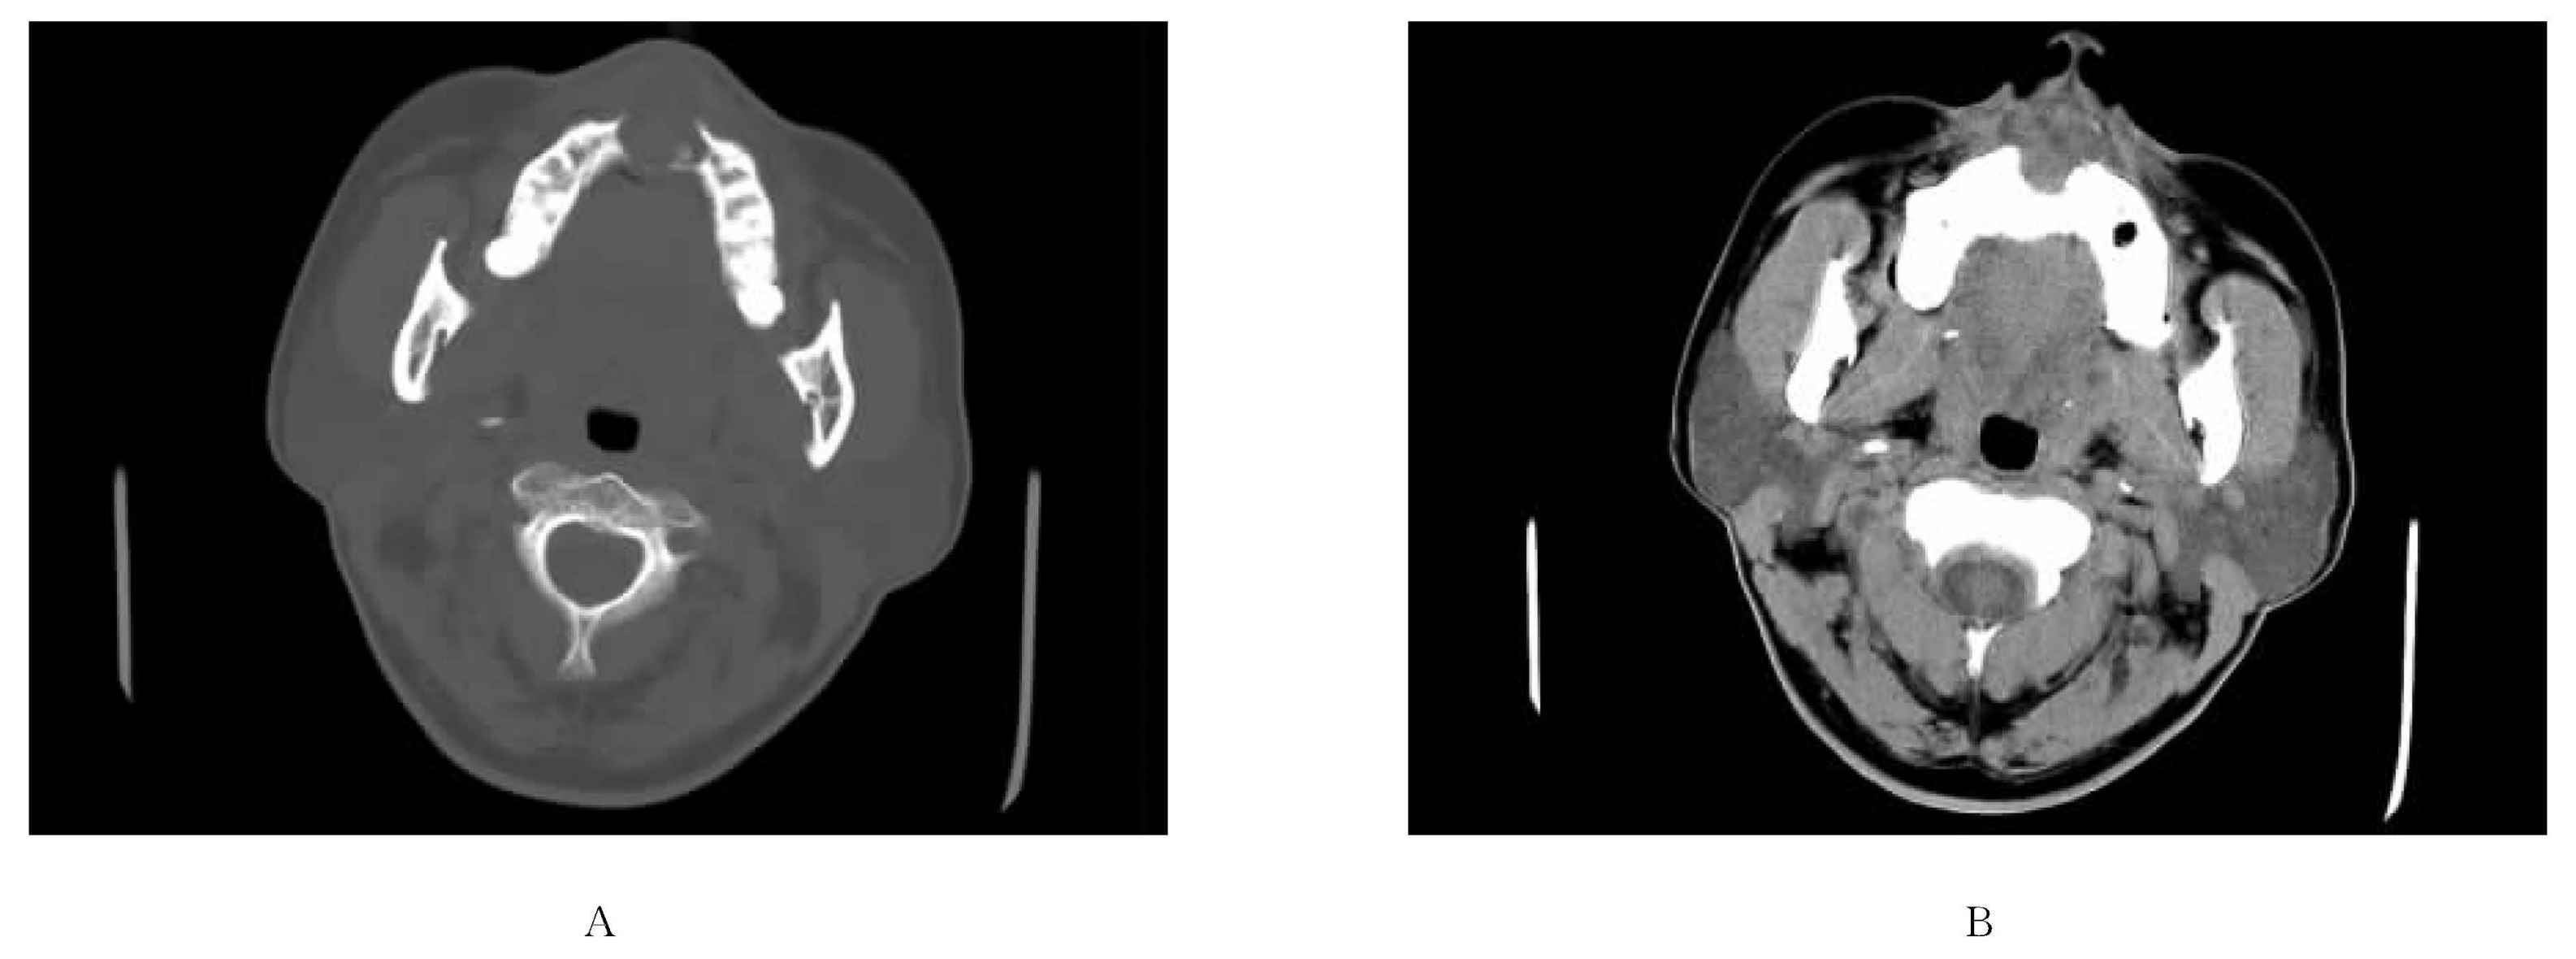
\includegraphics[width=.7\textwidth,height=\textheight,keepaspectratio]{./images/Image00154.jpg}
 \captionsetup{justification=centering}
 \caption{根尖囊肿\\{\small 上颌骨前部可见圆形低密度灶,边缘清晰锐利,其内有高密度牙根}}
 \label{fig7-1}
  \end{figure} 

\subsection{颌骨化脓性骨髓炎}

下颌骨化脓性骨髓炎较常见,而上颌骨相对少见。绝大多数为牙源性感染,占80%~90%;而血源性、外伤性感染仅占少数。血源性更多见于婴幼儿,且多发于上颌骨。

因其感染途径不同分为以下2种类型。

\subsubsection{中央型颌骨骨髓炎}

此型多见。是由病源牙首先引起根周或根尖周围组织感染,然后由颌骨中央向四周扩展,再累及骨皮质及骨膜的炎症过程。常见于下颌骨体部。炎症可局限或弥散,但弥散性现已不多见。

\textbf{【病因病理】}
致病菌通过病源牙牙髓腔或牙周进入根尖周引起感染,初期局部骨髓腔血管扩张,充血,局部骨质脱钙。进一步发展,局部骨质破坏形成脓肿。如果脓液向外扩散穿破颌骨的颊、舌侧密质骨,炎症就会局限而形成局限性骨髓炎;如果脓液沿骨髓腔扩散,则形成弥散性骨髓炎。由于各种原因导致的血运障碍,可形成小块或大块死骨。慢性期则有许多新骨形成。

\textbf{【临床表现】}
青壮年多见,男性多于女性。主要发生于下颌骨。起初炎症多局限,仅患牙痛,继之迅速波及邻牙、疼痛明显。牙周溢脓、口臭、下唇麻木、开口受限、面部肿胀,颌下淋巴结可肿大。并可有发热、头痛、全身不适等症状。如控制不利转入慢性期,主要表现有经久不愈的瘘管,有脓液溢出。发生于上颌骨者,症状轻微、局限,可并发上颌窦炎。

\textbf{【影像学表现】}
在发病第10~14天后才能显示骨质的病理变化,骨质变化分为4期:①弥散性破坏期:骨小梁模糊,骨质弥散性点状、斑点状和片状破坏,有骨膜反应。②病变局限期:炎症周围界限逐渐清晰,骨破坏区内多有大小、数量不等的分离或未完全分离的死骨,死骨一般密度较高(图\ref{fig7-2})。③新骨显著形成期:病灶明显局限,因病灶周围骨小梁变粗、数目增多而形成致密影像。如有死骨可见完全分离。④痊愈期:破坏区已被修复,修复区呈致密影像,无残腔和死骨。下颌骨外形有明显改变。此外,本型骨膜反应多较轻微,软组织肿胀多较显著。

\begin{figure}[!htbp]
 \centering
 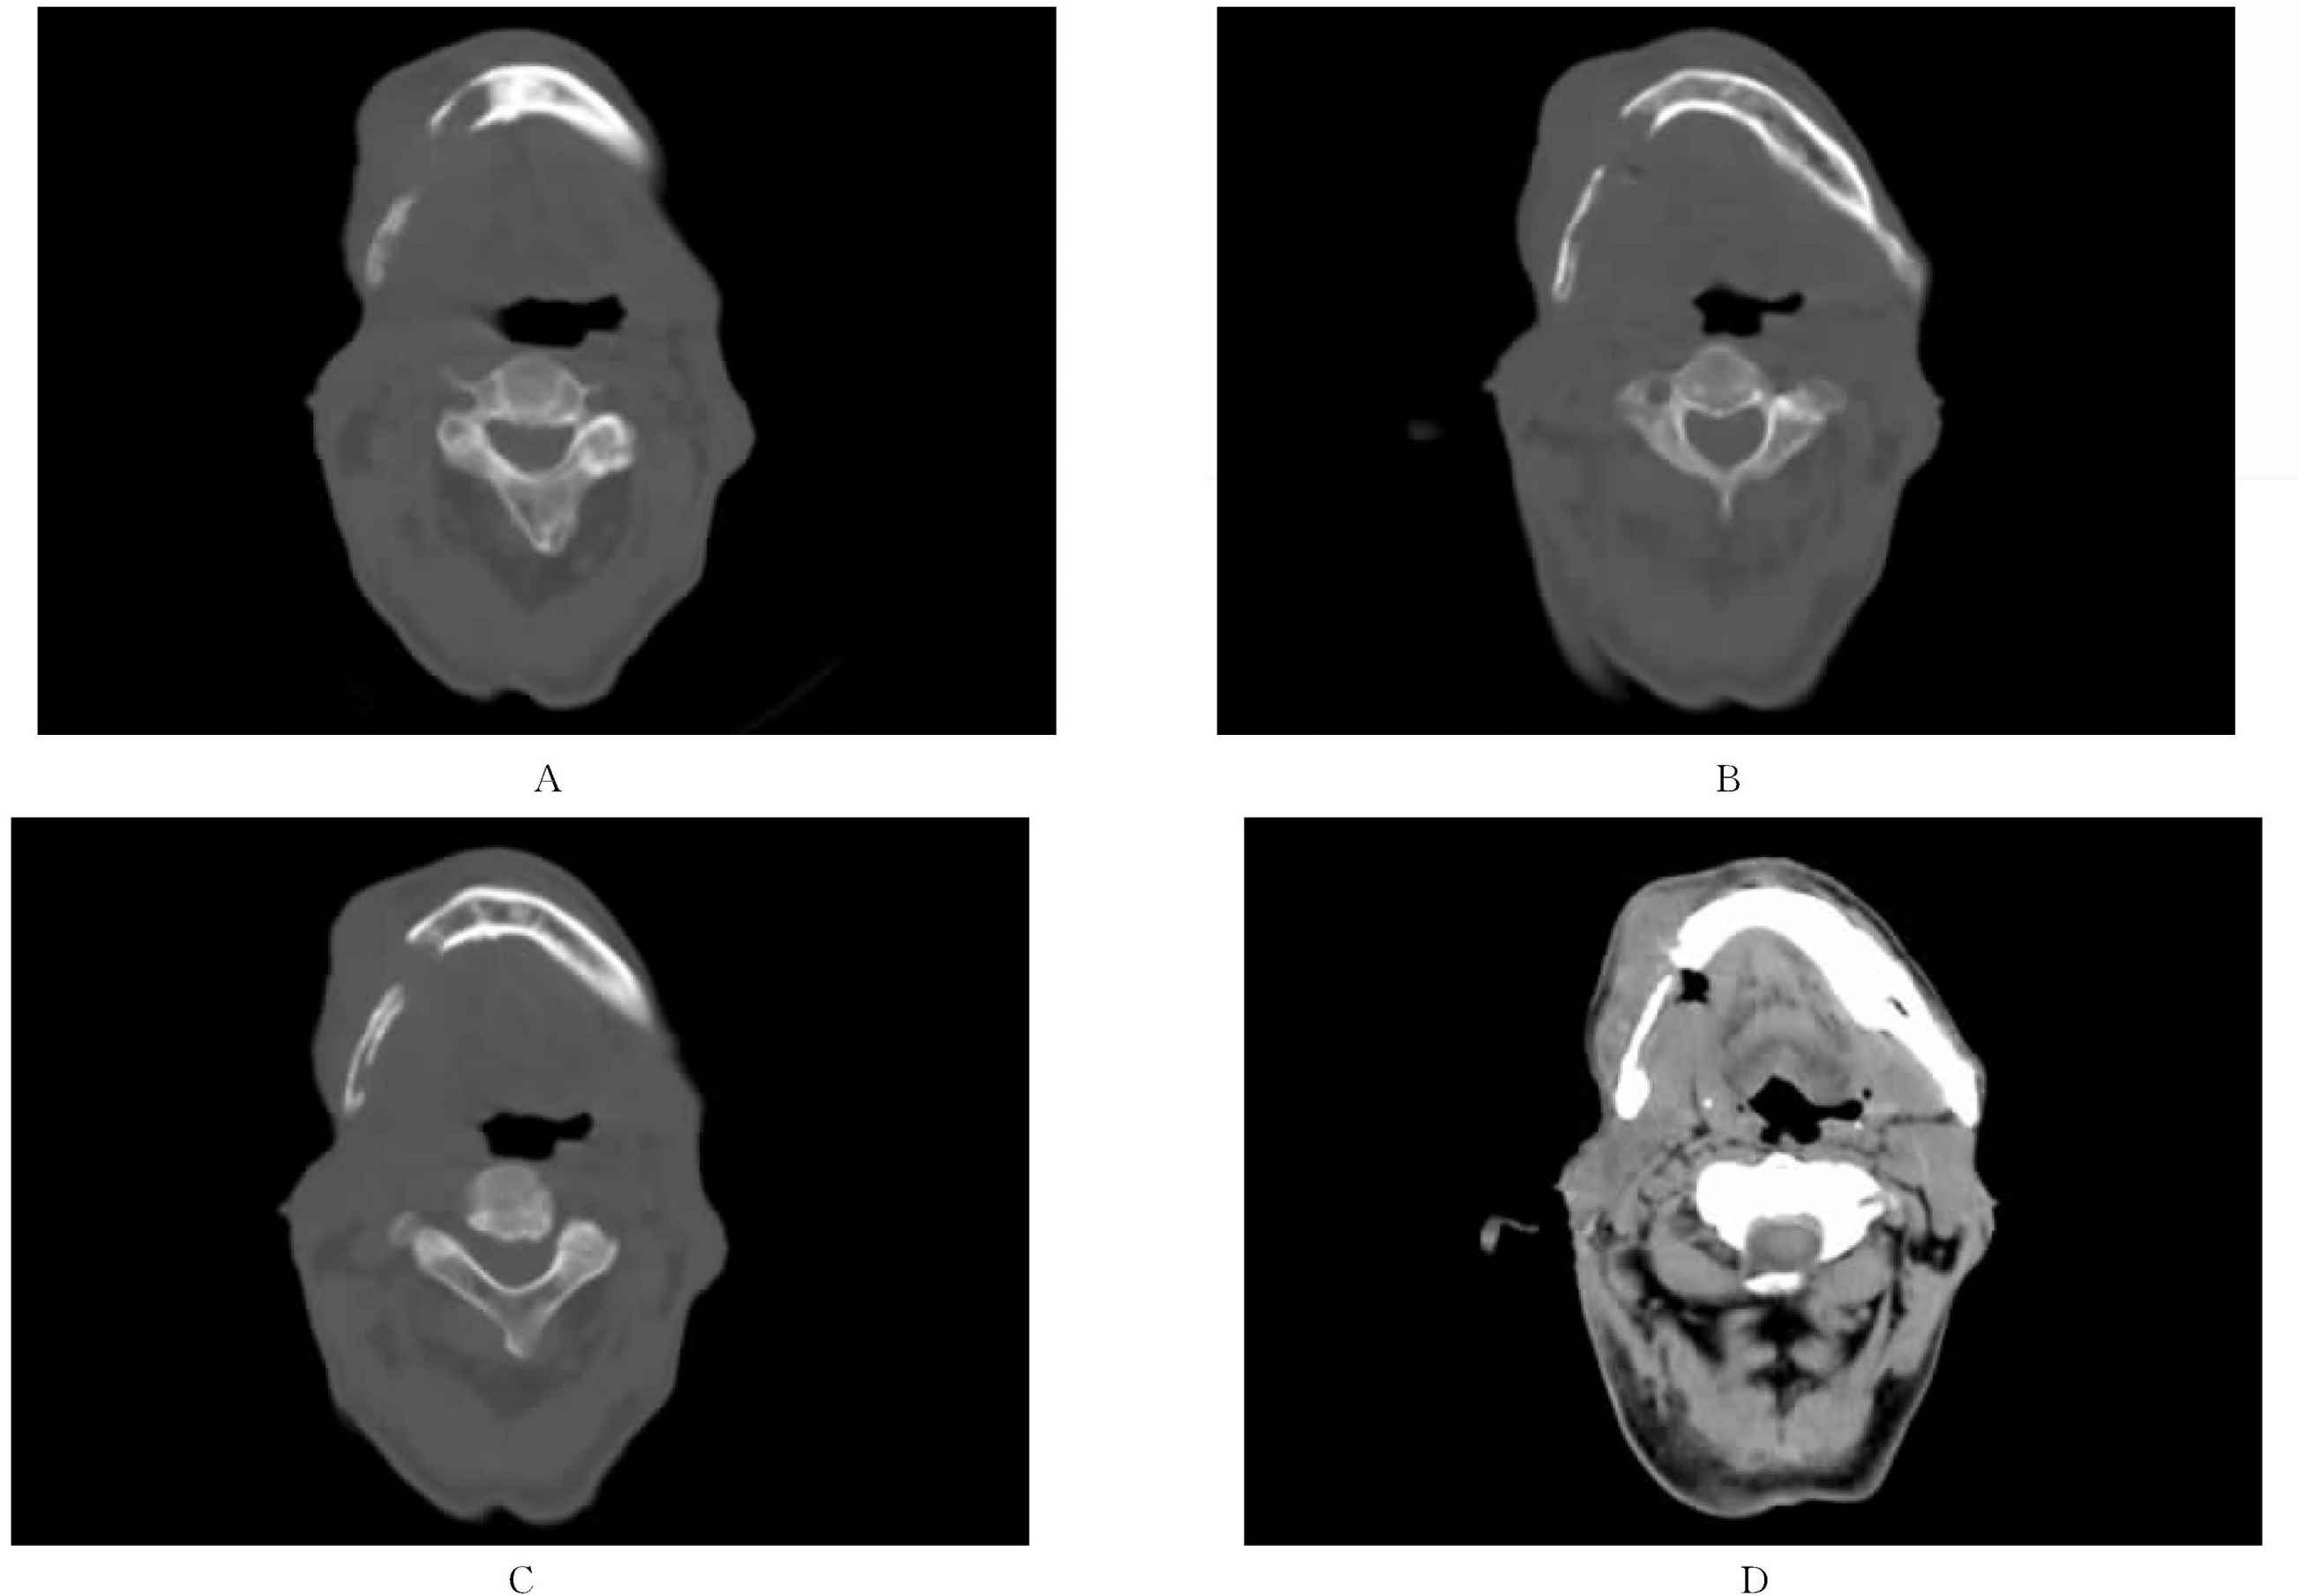
\includegraphics[width=.7\textwidth,height=\textheight,keepaspectratio]{./images/Image00155.jpg}
 \captionsetup{justification=centering}
 \caption{右侧下颌骨骨髓炎\\{\small 右侧下颌骨骨质破坏,边缘较清晰,局部有小死骨,邻近软组织肿胀,并有低密度气泡影}}
 \label{fig7-2}
  \end{figure} 

\textbf{【鉴别诊断】}
本型所引起的局限性骨质破坏需与牙龈癌侵蚀骨等恶性肿瘤相鉴别。牙龈癌表现为扇形不规则骨质破坏,一般无死骨及破坏区周围骨质增生,患牙浮在骨质破坏区内;临床上局部有软组织肿块。

\subsubsection{边缘型颌骨骨髓炎}

本病是由病源牙首先引起颌周间隙感染,进而侵犯骨膜、骨皮质乃至骨髓的炎症过程。此外,慢性低毒性的根尖周炎也能刺激颌骨体的骨膜形成新骨。多位于下颌升支、下颌角及第三磨牙区。

\textbf{【病因病理】}
感染主要起源于下颌第三磨牙冠周炎,也可由其他病牙引起。一般先发生颌周间隙感染,脓性渗出物刺激骨膜引起骨膜下成骨。大量的脓液积聚也可使局部骨膜溶解破坏、缺损,甚至密质骨及附近骨小梁破坏消失。有时脓性渗出物可沿哈佛管到达骨髓腔边缘部分。

\textbf{【临床表现】}
青少年多见,常有冠周炎或其他牙痛史。主要为腮腺咬肌区或颌周肿胀、炎性浸润,不同程度的开口受限及局部压痛。局部可有经久不愈的瘘管。由于感染局限,故一般全身症状不明显。

\textbf{【影像学表现】}
主要表现为骨质增生,骨质破坏甚少。可见弥漫性骨密度增高。增生的边缘一般较整齐,且骨皮质无明显破坏或破坏轻微,一般无死骨形成。早期偶有线状骨膜反应。

\textbf{【鉴别诊断】}
本型在有明显骨质增生时需与成骨肉瘤相鉴别。前者升支外侧骨皮质无明显破坏;后者升支外侧骨皮质常有广泛破坏,骨皮质外骨膜增生和肿瘤骨缺乏整齐的外缘,有时放射状瘤骨可穿入软组织肿块内。

\subsection{下颌骨弥散性硬化性骨髓炎}

本病命名混乱,还称为慢性硬化性非化脓性骨髓炎、骨化骨髓炎、干性骨髓炎、原发性骨髓炎等。

\textbf{【病因病理】}
尽管多认为由低毒性感染所致,但炎症的起因并不明确。很多病例细菌培养和其他病原体是阴性。国外有学者注意厌氧菌培养,并发现痤疮丙酸菌和中间型消化链球菌在一些病例中是重要原因。细菌很可能是通过根管感染而影响骨组织和血管系统。慢性疾病过程可能与内源性感染和激发机体的免疫反应有关。

\textbf{【临床表现】}
可发生于任何年龄,但以成人多见,多认为女性多与男性。最常见的症状为反复疼痛和肿胀,间断性加重,可反复持续数年。抗炎治疗效果不佳。急性发作可伴有张口困难和咬肌区肿胀。病变严重时可有低热、血沉加快、白细胞计数升高。瘘道和局部脓肿形成很少见。可有颌下淋巴结肿大。

\textbf{【影像学表现】}
早期(起病后1~2个月)在下颌骨(下颌体、角部)下缘有轻度的局限性密度减低区和致密区相混杂,表明有少量骨质破坏,同时有骨膜增生和骨膜成骨,可类似恶性肿瘤的表现。这种骨缺损和硬化也可侵犯升支、髁状突。这种侵犯少数在1~2年内自行消失。但通常在几年内缓慢进展。在年轻人中,可见下颌骨体积增大,主要是厚度增加为主;在年龄较大者中,有时可见体积有减小的趋势(特别在下颌角区),而髁状突常变大,角前切迹宽度变小。此外,临床症状加重时,常倾向于骨溶解破坏;而症状缓解时溶骨区缩小甚至消失;当急性发作次数变得很少时,骨硬化变得更显著且界限不清。在病变区可有界限不清的小的溶骨,5~10年后硬化消失,骨结构恢复正常。

\textbf{【鉴别诊断】}
本病与边缘性颌骨骨髓炎、成骨肉瘤、骨纤维异常增殖症、畸形性骨炎、弥漫性巨大牙骨质瘤临床和影像学有相似之处,应注意鉴别。

\subsection{颌面骨结核}

颌面骨结核少见,不到全身骨结核的0.2%。其中又以颌骨及颧骨多见。

\textbf{【病因病理】}
颌骨结核的感染可以是口腔黏膜、牙龈的病变蔓延至颌骨,或痰液中的结核菌经拔牙创口直接侵入骨内,但上述途径很少。较多见的感染途径还是其他脏器结核的血行感染至颌面骨。经血循环停留在松质骨内的结核菌,起初引起非特异性反应,随即形成结核结节,进而干酪坏死,并逐渐融合。随着病变发展,骨质逐渐被破坏,并被脓液所代替。大量脓液产生,成为冷脓肿,如经皮肤破溃即形成窦道,随后可继发化脓菌感染。

\textbf{【临床表现】}
由口腔黏膜、牙龈的结核蔓延至颌骨者,主要表现为局部溃疡呈缓慢发展、疼痛、无自愈倾向。也可破坏牙槽骨,致患牙松动,甚至脱落。血行感染者多见于下颌角及颧颌缝。初期表现为局部无痛性肿胀,或有间歇痛。进一步发展可波及局部口腔黏膜及皮肤,形成冷脓肿,进而可遗留经久不愈的瘘管。全身症状不明显,一般仅有低热和血沉增快。

\textbf{【影像学表现】}
①由口腔黏膜、牙龈的结核直接扩散而侵犯颌骨者,可见局部骨质破坏,也可有小死骨形成。继发感染可有骨质增生。②侵犯下颌骨的病变,可见局部低密度区,以骨破坏为主,无骨质增生,这是颌骨结核的特点。继发感染破坏区边缘骨质增生时,病灶边界清楚。虽有死骨形成,但较细小。③儿童患者可有骨膨胀性改变、牙胚移位甚至坏死。成人骨质坚实,故骨膨胀较少见。④下颌角是下颌骨结核的好发部位。其破坏区远离牙根,无病源牙,这与牙源性骨髓炎不同。⑤发生于颧颌缝的结核多侵犯该缝以下的上颌骨部分,但上颌窦一般不受累。

\subsection{颌骨放线菌病}

本病少见,是由放线菌引起的慢性化脓性特异性颌骨炎症。

\textbf{【病因病理】}
原发者罕见,多为存在于正常人龋洞、龈袋、扁桃体窝等处的放线菌,在机体抵抗力低时,通过损伤的黏膜、拔牙创面、冠周炎等途径侵入颌面部而发病。下颌骨较上颌骨多见。病理学特征是在脓液或肉芽组织中出现菌体及菌丝形成的黄色小颗粒(称为“硫黄颗粒”)。

\textbf{【临床表现】}
多见于青壮年男性。常见于下颌骨后部。病变进展缓慢、病程长。可有张口受限。炎性病灶软化形成脓肿后,局部皮肤呈鲜红或紫红。脓肿破溃后有少量脓液溢出,并可形成窦道或瘘管。也可只有颌骨中央损害,而颌周软组织不受侵犯。

\textbf{【影像学表现】}
其X线和CT主要改变是骨质破坏及周围的骨质呈反应性新骨增生。由于骨质破坏与增生的程度不同,可呈各种不同表现。因为病变多累及骨膜,并引起骨膜成骨而导致骨质明显增厚、增宽、膨隆畸形。因骨内有脓腔或肉芽而使其间有大小不等、数目不同的骨质破坏灶或因脓瘘相互通连呈多处条状沟纹及窦道影。单纯表现为骨膜成骨或病变部的骨质疏松或较大的骨质破坏区则很少见。

\subsection{颌骨放射性骨坏死}

放射线或其他放射能的作用,使骨组织发生无菌坏死,叫放射性骨坏死。一旦坏死的骨组织因为继发感染而发生炎症,则称为放射性骨髓炎。

\textbf{【病因病理】}
其病因病理尚有争议。普遍认为放射、创伤和感染是颌骨放射性骨坏死的三大发病因素。骨坏死的机制为:照射区内小动脉的损伤导致骨组织血运障碍和放射线直接对骨细胞的损害。骨膜对放射线高度敏感,表现为肿胀、增厚、易剥离,骨膜内面明显玻璃样变,成骨细胞层破坏,丧失沉积新骨能力。

\textbf{【临床表现】}
主要症状是疼痛,多为间歇性,也可深部持续性剧痛,也有患者无疼痛症状。可有张口困难、口臭。骨坏死后易继发感染,创口不愈、溢脓,而形成经久不愈的瘘管。还可合并有面颊部软组织坏死。

\textbf{【影像学表现】}
颌骨放射性骨坏死的部位与对原发肿瘤的照射部位有关。①颌骨:病变早期骨质呈弥散性疏松,进而有斑点状、虫蚀样骨质破坏。稍晚时,其间有散在增粗的骨小梁和密度增高的小团块病理性骨沉积,二者界限明显,或在较均匀密度减低的背景中,增粗的骨小梁纵横交错呈网格状改变,或表现为密度均匀增高伴有散在点状低密度的改变。易继发感染而使病情加重,病灶常从牙槽突开始,表现为局部和根尖周密度减低,骨破坏区之外常有明显的硬化反应带。骨膜反应少见。②牙及牙周:放射性龋较多见,好发于牙颈部,常进展较快。偶尔可见牙内吸收。还可有牙周膜间隙增宽、骨硬板密度减低或消失,牙槽突吸收、高度降低等。

\textbf{【鉴别诊断】}
①恶性肿瘤复发:放射性骨髓炎所引起的骨质破坏可与恶性肿瘤复发混淆。后者X线或CT可见骨质破坏迅速,且骨质破坏不限于放射野内;临床上可扪及肿块。②牙源性骨髓炎:放射性骨髓炎如照射区内有牙齿,且骨质破坏从牙槽突开始,有时不易与牙源性骨髓炎鉴别。主要应结合病史加以鉴别。

此外,应注意结合病史与颌骨化学性坏死(主要原因是磷、砷、汞等化学物质的中毒)相鉴别。

\subsection{颌骨肿瘤与肿瘤样病变的分类}

颌骨肿瘤可来源于成牙组织,也可来源于颌骨的成骨组织、纤维组织、脉管组织和骨髓组织等(见表\ref{tab7-1})。

\begin{table}[htbp]
\centering
\caption{颌骨肿瘤与肿瘤样病变的分类}
\label{tab7-1}
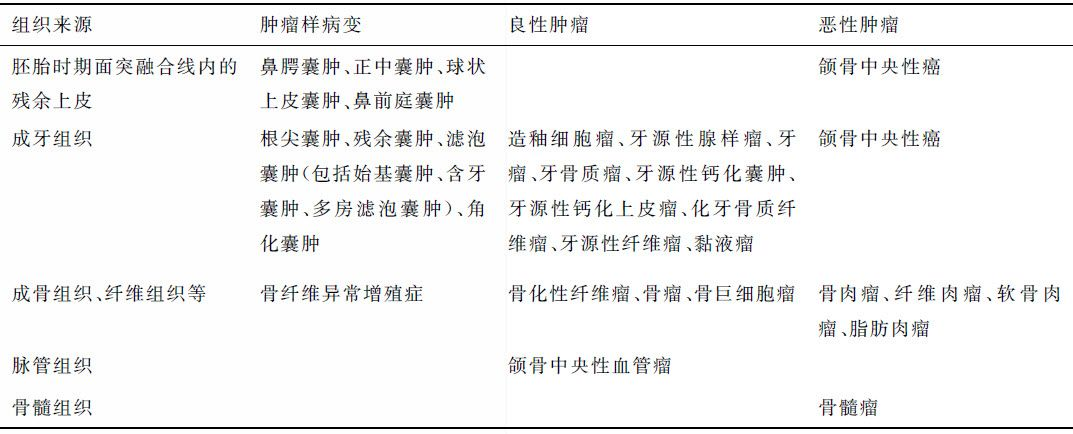
\includegraphics[width=\textwidth,height=\textheight,keepaspectratio]{./images/Image00156.jpg}
\end{table}

颌骨囊肿根据组织来源和发病部位分为2类:①由成牙组织而来的颌骨囊肿,称为牙源性囊肿。②由胚胎发育过程中残存于面突连接处的上皮发展而来的囊肿,称为面裂囊肿或非牙源性囊肿。面裂囊肿都有其特定的部位和形状,与牙齿关系不大。根据发病部位可分为鼻前庭囊肿、鼻腭管囊肿、正中囊肿和球状上颌囊肿,其中以鼻前庭囊肿最常见。

\subsection{根尖囊肿和残余囊肿}

根尖囊肿亦称根端囊肿、齿根囊肿,为最常见的颌骨囊肿。其病因是牙周膜及附近牙槽骨的牙周上皮残余,因慢性炎症的刺激引起上皮增生,在中心部发生液化而形成囊肿。残余囊肿占颌骨囊肿的第二位,其成因与根尖囊肿相同,是在拔牙后残余上皮形成的。

\textbf{【影像学表现】}
以X线检查为优,其特点是以病源牙包括深龋、残根、死髓牙的牙根为中心的单房性均一低密度囊腔。大小不一,膨胀性生长,边缘硬化清晰、无残缺。该牙的牙周膜与硬骨板消失,邻近牙根被推移,亦可突入囊中(见图\ref{fig7-1})。发生于上颌骨中,可有上颌窦推移,亦可发生于上颌窦内。继发感染则囊壁、硬化环模糊或有破坏表现,囊内密度增高。

残余囊肿是在拔牙后的牙槽窝下方颌骨内呈现均一低密度囊腔,以此可与根尖囊肿相区别。如将所谓来自牙齿发育后残留的鳞状上皮脱屑形成的囊肿亦归为残余囊肿,则残余囊肿与根尖囊肿将无法区别。

\subsection{滤泡囊肿}

滤泡囊肿包括始基囊肿、含牙囊肿和多房滤泡囊肿。

\textbf{【病因病理】}
上述囊肿均为牙齿发育过程中,在炎症刺激或创伤激惹等因素影响下,造釉器星网状层变性,牙滤泡周围液体渗出形成的囊肿。囊肿多位于下颌角磨牙区,尤以第三磨牙区多见。①始基囊肿:又称为单纯滤泡囊肿。但WHO将始基囊肿改称为角化囊肿。好发于下颌角第三磨牙处,该牙常缺如。因囊肿发生于牙胚早期,即造釉器尚未分化成釉质阶段,因此囊内无牙可见。②含牙囊肿:发生于未萌出的牙胚晚期,造釉器已基本分化成釉质,即牙齿硬组织已基本形成,故囊肿内含有牙齿。囊肿是因造釉器星网状层变性,牙滤泡周围液体渗出至牙冠与上皮之间形成,故牙冠被包入囊内,牙根居囊外。囊内牙齿为正常牙或畸形牙。③多房滤泡囊肿:临床并不多见。囊腔呈多房,含牙或不含牙。

\textbf{【临床表现】}
可发生于任何年龄,以青壮年多见。男多于女。临床常可见缺牙伴第三磨牙区颌骨膨隆。

\textbf{【影像学表现】}

1.始基囊肿:好发于下颌角第三磨牙处,囊肿占据牙的位置,呈圆形或椭圆形近水样均匀低密度区,囊肿较小,边缘光整、有硬化圈,囊内无牙或牙胚。亦不与其他牙齿相接触。

2.含牙囊肿:早期常表现为下颌第三磨牙的冠周围间隙增宽(说明该牙造釉器的星网状层已开始变性),继而冠周围间隙增大而形成圆形近水样均匀低密度区。其边缘清晰锐利,囊壁与牙颈部相连,牙冠全部包入囊肿,牙根居囊外。若囊肿继续长大,亦可将整个牙齿包入囊内。

3.多房滤泡囊肿:好发于下颌角的磨牙区,常向下颌角及升支发展。典型者局部呈多房性囊状近水样均匀低密度区。囊腔大小差异不大。囊壁光滑锐利,完整无缺,有硬化圈。囊肿波及牙根,一般无牙根吸收表现。囊内多半无牙齿,如囊内有牙齿则囊和牙的关系与含牙囊肿相同。

\subsection{牙源性角化囊肿}

本病亦为较常见的牙源性囊肿,具有明显的复发倾向、侵袭性生物学行为以及潜在的肿瘤性质。

\textbf{【病因病理】}
关于其来源意见不一,多数人认为来源于牙板残余或原始滤泡,因此认为牙源性角化囊肿即始基囊肿。1971年,WHO在国际肿瘤分类中,将始基囊肿改称为角化囊肿。但有些学者认为二者有别。角化囊肿含有大量的角化物,表面覆有不全角化或正常角化层。该囊肿易继发感染,有转变为造釉细胞瘤和发生恶变的可能。约10%具有多发性。

牙源性角化囊肿可为单发,亦可多发。如同时伴有基底细胞痣或癌及分叉肋等病者,称为基底细胞痣综合征或痣样基底细胞癌综合征。本综合征常有家族史,被认为是常染色体显性遗传病。

\textbf{【临床表现】}
可发生于任何年龄,但有两个高峰期即20~30岁和50岁年龄组。男多于女。有些患者与遗传因素有明显关系。早期多无症状,随病变发展可有颌骨膨胀。临床上有一定复发倾向。

\textbf{【影像学表现】}
X线或CT可见:下颌多于上颌。囊肿多位于下颌骨之磨牙区,尤以下颌升支及体部多见。发生于上颌骨者以磨牙区多见,但亦可位于前牙区。囊肿常单发,多发者少见。其影像学表现差异大,缺乏特征性。位于下颌骨者易沿颌骨长轴生长而呈长椭圆形,亦可呈分房状或边缘有多发骨嵴。位于上颌骨者常突入上颌窦。由于生长活跃,部分病例囊壁周围骨硬化缘不完整,并可见骨质缺损,与造釉细胞瘤相似。由于囊内含蛋白角化物,故囊内密度常呈混杂密度。囊肿内含牙或不含牙(含牙者可能为含牙囊肿演变而来,不含牙者可能为始基囊肿演变而来),牙根可有斜面状、锯齿状吸收,与造釉细胞瘤很相似。本病侵袭性强,波及范围较其他囊肿大,常沿颌骨长轴发展。下颌骨者膨胀多向舌侧,上颌骨者多突向唇颊侧或颌间间隙,并均可穿破骨皮质。此外,本病具有复发性,并可恶变呈边缘模糊的溶骨性破坏。

基底细胞痣综合征的影像学表现:除颌骨囊性尤其多发性囊性病变外,尚可见:①大脑镰、小脑幕或蝶鞍韧带钙化;②肋骨分叉;③脊柱弯曲或椎体及附件畸形。

\subsection{面裂囊肿}

\subsubsection{鼻前庭囊肿}

本病亦称为鼻牙槽突囊肿、鼻底囊肿、鼻黏液囊肿等,为最常见的面裂囊肿。

\textbf{【病因】}
鼻前庭囊肿的病因不清。早期认为是潴留囊肿,即鼻底黏膜黏液腺管阻塞所致,还有人认为起源于鼻泪管的残余上皮。目前多认为起源于裂隙发育性残余上皮,在胚胎形成时起源于残余的上皮细胞或者由于包埋上皮增生而形成,沿着上颌、内鼻和外鼻突融合部发生。机械刺激、炎性或外伤是重要诱发因素。

\textbf{【临床表现】}
发病年龄多在40~50岁之间,多见于女性,多为单侧发病。位于由鼻翼围成的鼻前庭底部皮下、梨状孔之前外方。早期多无症状。随病变发展感鼻翼根部膨隆、胀满感,合并感染可有局部红、肿、热、痛。

\textbf{【CT表现】}
边缘清楚的囊性病灶,CT值较一般囊肿高,继发感染时边缘不清。一般无骨质改变,大时可压迫上颌骨额突,轻者仅表现为骨质硬化凹陷,重者可出现明显压迹。

\subsubsection{鼻腭管囊肿}

本病亦称切牙管囊肿。

\textbf{【病因】}
来自鼻腭管(切牙管)上皮,位于切牙管内。也是非牙源性囊肿较常见者。

\textbf{【临床表现】}
发病年龄多在30~60岁,男女比例约3∶1。最常见的表现是腭中线前方局部隆起。

\textbf{【CT表现】}
正常切牙管宽<5mm。该囊肿表现为位于中切牙之间或见切牙管扩大的低密度区,呈卵圆形或心形,边缘清楚、硬化(图\ref{fig7-3})。两个中切牙牙根多被推开,但X线可见牙周膜和硬骨板的连续性存在。

\begin{figure}[!htbp]
 \centering
 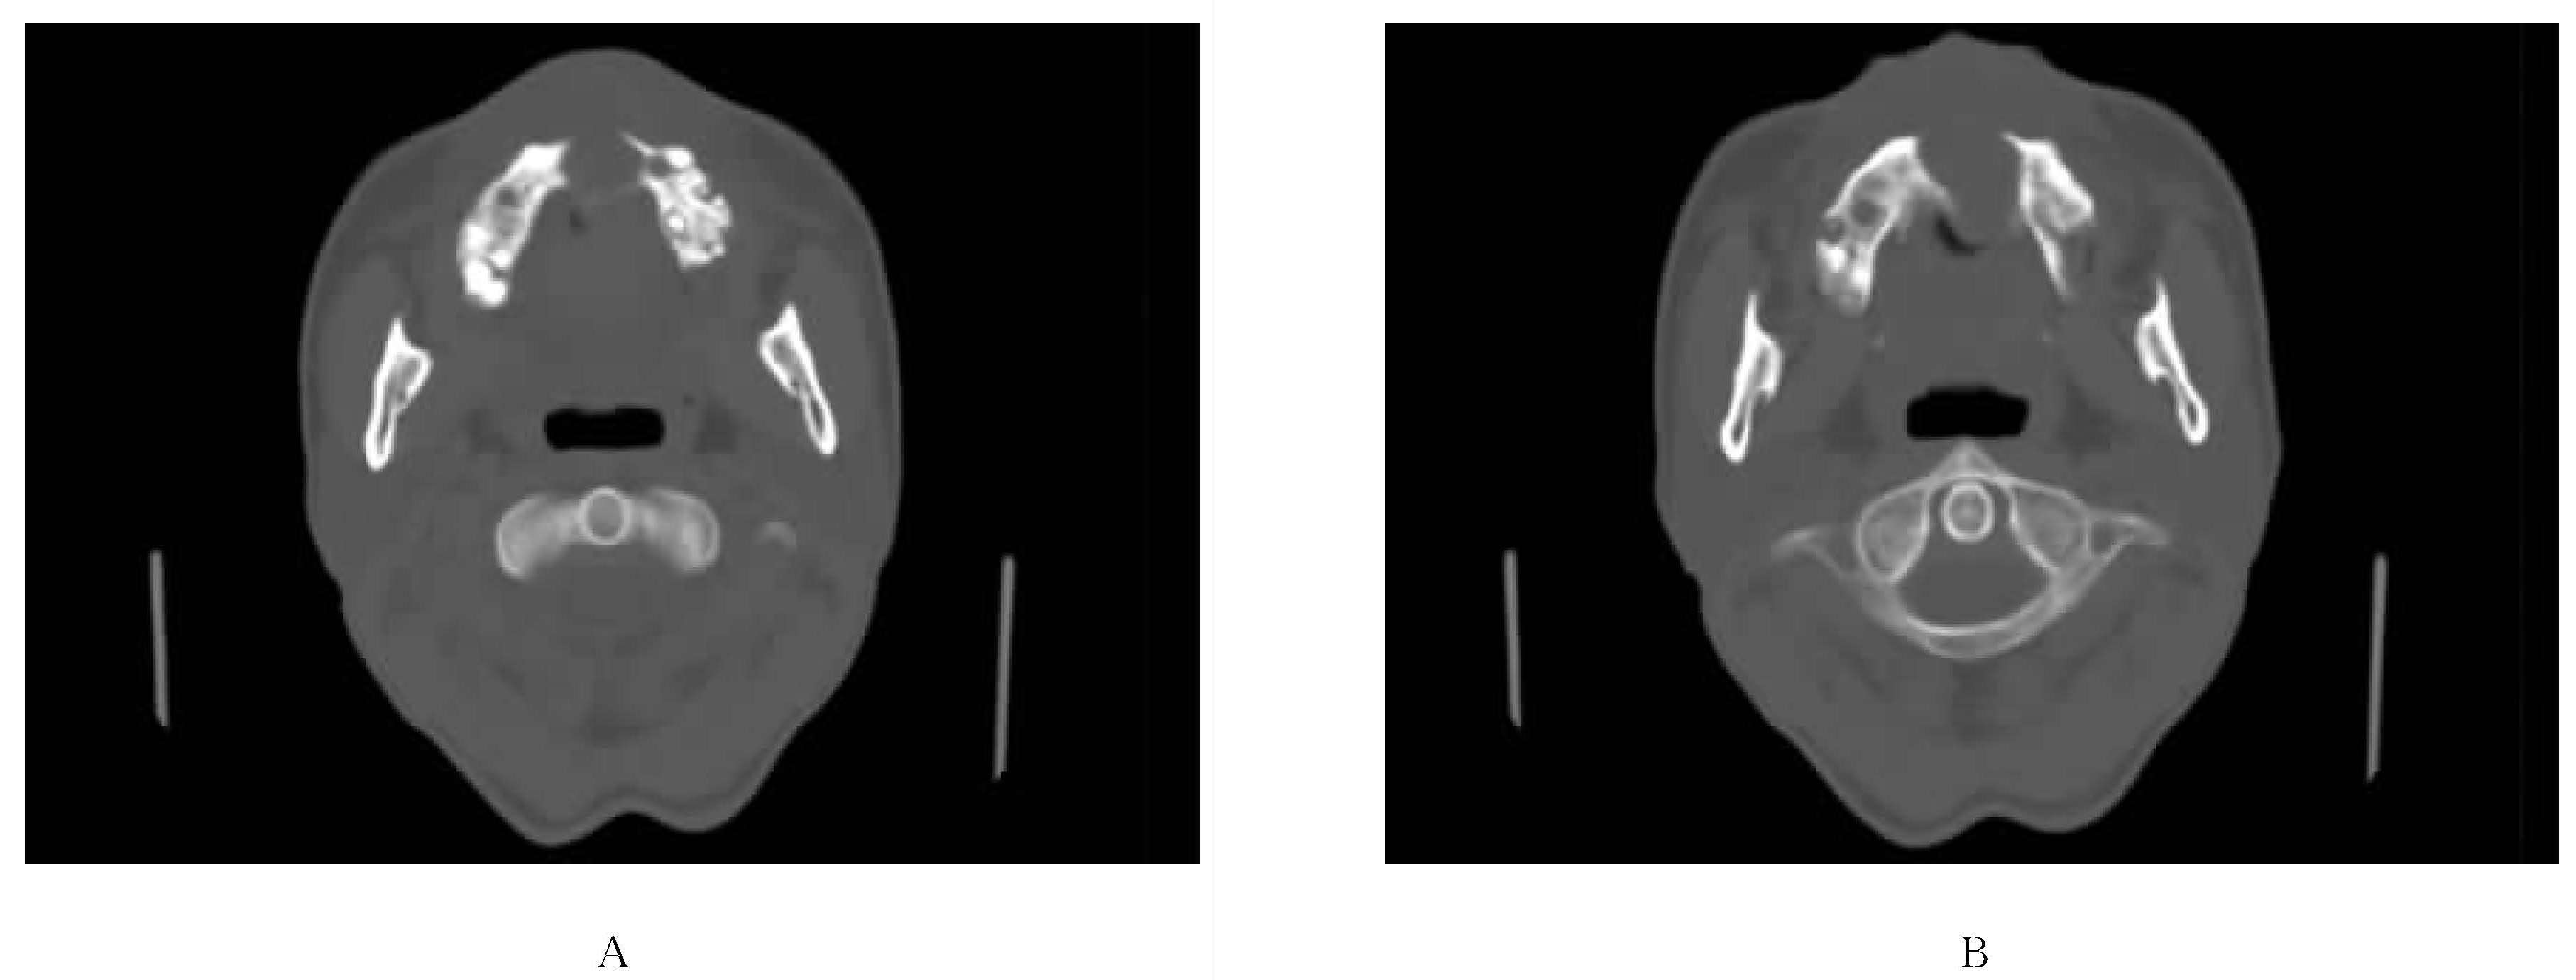
\includegraphics[width=.7\textwidth,height=\textheight,keepaspectratio]{./images/Image00157.jpg}
 \captionsetup{justification=centering}
 \caption{切牙管囊肿\\{\small 上颌骨前部有圆形低密度灶,界限清晰(手术证实)}}
 \label{fig7-3}
  \end{figure} 

\subsubsection{正中囊肿}

本病亦称腭正中囊肿、上颌正中囊肿。

\textbf{【病因】}
来自胚胎时期两侧上颌骨腭突之间的上皮。此外,有人将来自胚胎时期下颌突之间上皮的、位于下颌正中线处的圆形囊肿称为下颌正中囊肿。

\textbf{【临床表现】}
上颌正中囊肿表现切牙管之后、上颌骨之腭中线区局部隆起、不适。下颌正中囊肿表现为下颌正中处局部隆起、不适。

\textbf{【CT表现】}
上颌正中囊肿位于切牙管之后、上颌骨之腭中缝的任何部位。呈边界清楚、局限的低密度区。多呈圆形,边缘硬化。下颌正中囊肿位于下颌正中线处的圆形低密度区,边缘硬化。囊肿均与牙齿无关。

\subsubsection{球状上颌囊肿}

本病亦称球颌囊肿。

\textbf{【病因】}
来自胚胎期球状突与上颌突之间的上皮。位于上颌侧切牙与尖牙之间。

\textbf{【临床表现】} 上颌侧切牙与尖牙之间处局部隆起、不适。

\textbf{【CT表现】}
表现为上颌侧切牙与尖牙(均为活髓牙)之间,边缘清楚的、局限性低密度区,呈倒置的梨形,边缘有硬化。侧切牙与尖牙牙根被推开。

\subsection{造釉细胞瘤}

本病又称为成釉细胞瘤,是最常见的牙源性肿瘤。目前临床及病理学医师多主张造釉细胞瘤是一种低度恶性肿瘤。造釉细胞瘤确实易复发并发生恶变。

\textbf{【病理】}
组织来源主要为牙源性上皮,即残余的牙板、造釉器;少数来源于牙源性囊肿上皮和口腔黏膜上皮。肿瘤大小不等。巨检剖面分为实质型与囊肿型,后者分为单房和多房两类。肿瘤有包膜,但不完整。一般认为早期为实质型,以上皮细胞增殖为主,随进展退化,囊变成囊肿型。肿瘤继续生长亦可使囊肿型变为实质型。镜下部分瘤细胞分化不良,具有潜在或低度恶性表现。

\textbf{【临床表现】}
多发生于青壮年,男女发病相近,下颌比上颌多,以下颌体部及角部多见。生长缓慢,初期无自觉症状,逐渐发展可使颌骨膨大。肿瘤侵犯牙槽突时可使牙松动、移位和脱落。一般无神经症状,无开口受限。手术不彻底者易复发。

\textbf{【影像学表现】}
其表现多样。CT表现肿瘤呈低、等密度混合的囊状区,可为多房状、蜂窝状或单房状。颌骨膨大、皮质变薄。CT可清晰显示骨外软组织肿块。增强扫描病灶实性部分明显强化。

1.实质型:此型很少见。表现为蜂窝状、砂粒状低密度区,颌骨边缘皮质可被吸收而不完整,故有砂粒型和蜂窝型之称。罕见的表现有颌骨膨大,密度增高。

2.多房型:此型多见。囊腔大小不一,成群排列,相互重叠或呈囊套囊表现。囊腔大小差别越大,则越应视为造釉细胞瘤。大的囊腔位于下颌支时常为造釉细胞瘤。囊壁为线状硬化圈,其边缘呈分叶状,有切迹及残缺、中断表现。颌骨可显著膨大,骨皮质变薄甚至中断,且可形成软组织肿块。囊腔内有无牙齿及牙的形态取决于局部牙本身造釉器发育成熟的程度(所含牙可为埋伏牙、阻生牙、额外牙)。邻近牙根可呈锯齿状或截断状吸收,或压迫移位及脱落。囊变区内密度不均,其内常可见软组织密度及细小斑点状钙化。

3.单房型:此型相对少见。瘤体呈单个类圆形囊腔,囊壁不光滑,并有分叶、切迹和中断。囊腔内多不含牙。瘤内密度不均,可有斑点状钙化。局部骨骼改变和邻近牙的变化与多囊型者相似(图\ref{fig7-4})。少数边缘光滑整齐、甚至含牙,与始基囊肿或含牙囊肿不易鉴别。

\begin{figure}[!htbp]
 \centering
 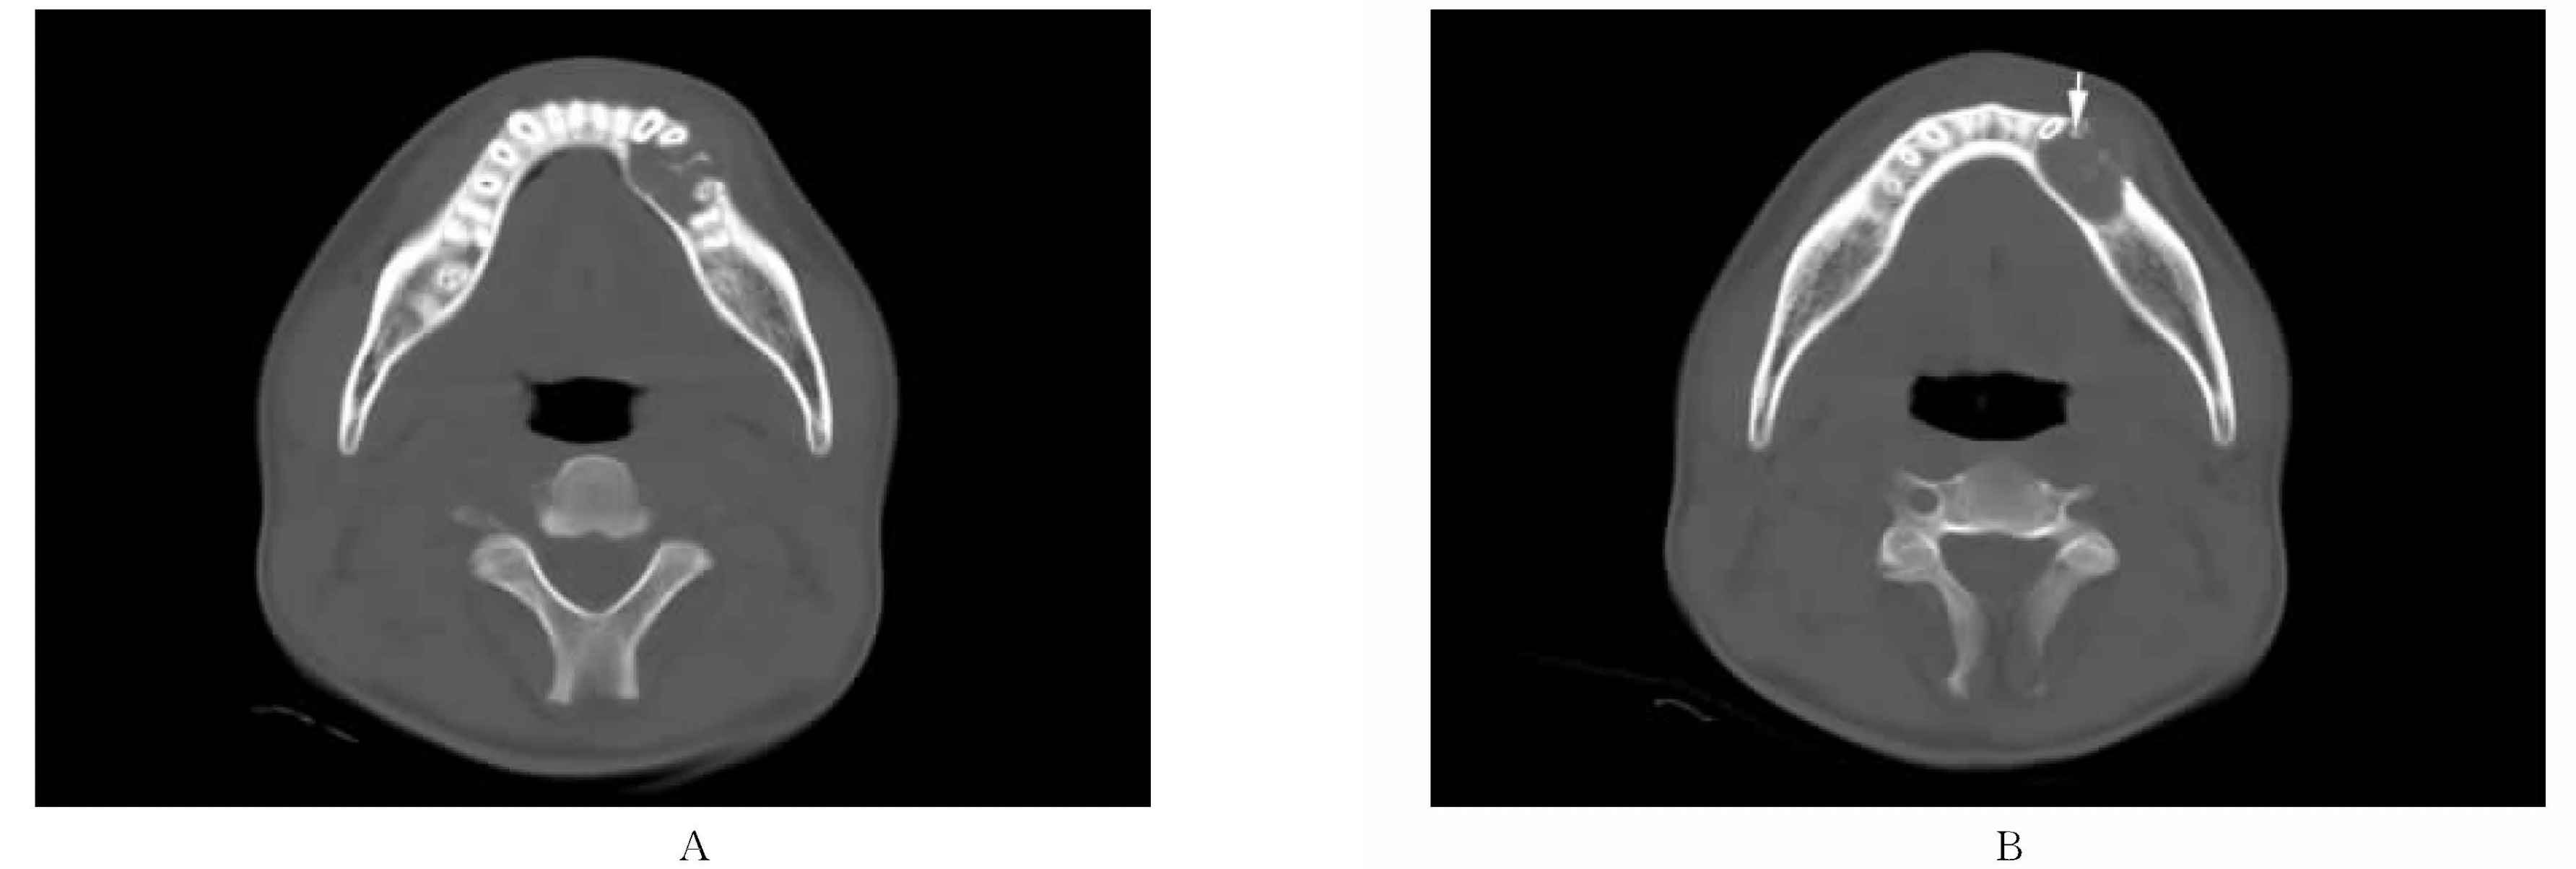
\includegraphics[width=.7\textwidth,height=\textheight,keepaspectratio]{./images/Image00158.jpg}
 \captionsetup{justification=centering}
 \caption{下颌骨造釉细胞瘤\\{\small 14岁男性。左侧下颌骨有囊状骨质破坏区,边缘有中断,其内有斑片状钙化。此外,A示左下第4、第5齿受压分离;B示左下第4齿根有吸收表现(箭)}}
 \label{fig7-4}
  \end{figure} 

恶变的影像学表现:早期为一般表现的囊腔。发生恶变后囊腔多消失,出现骨破坏表现。清晰的边缘变为模糊消失,进展迅速。骨皮质出现广泛侵蚀、破坏及突破,失去颌骨的形态。软组织肿块增大显著,密度增高。X线和CT颇似骨恶性肿瘤,但边缘尚可见残留的多房痕迹。

\textbf{【鉴别诊断】} 见表\ref{tab7-2}。

\begin{longtable}{c}
  \caption{颌骨造釉细胞瘤的鉴别诊断}
  \label{tab7-2}\\
  \endfirsthead
  \caption[]{颌骨造釉细胞瘤的鉴别诊断}
  \endhead
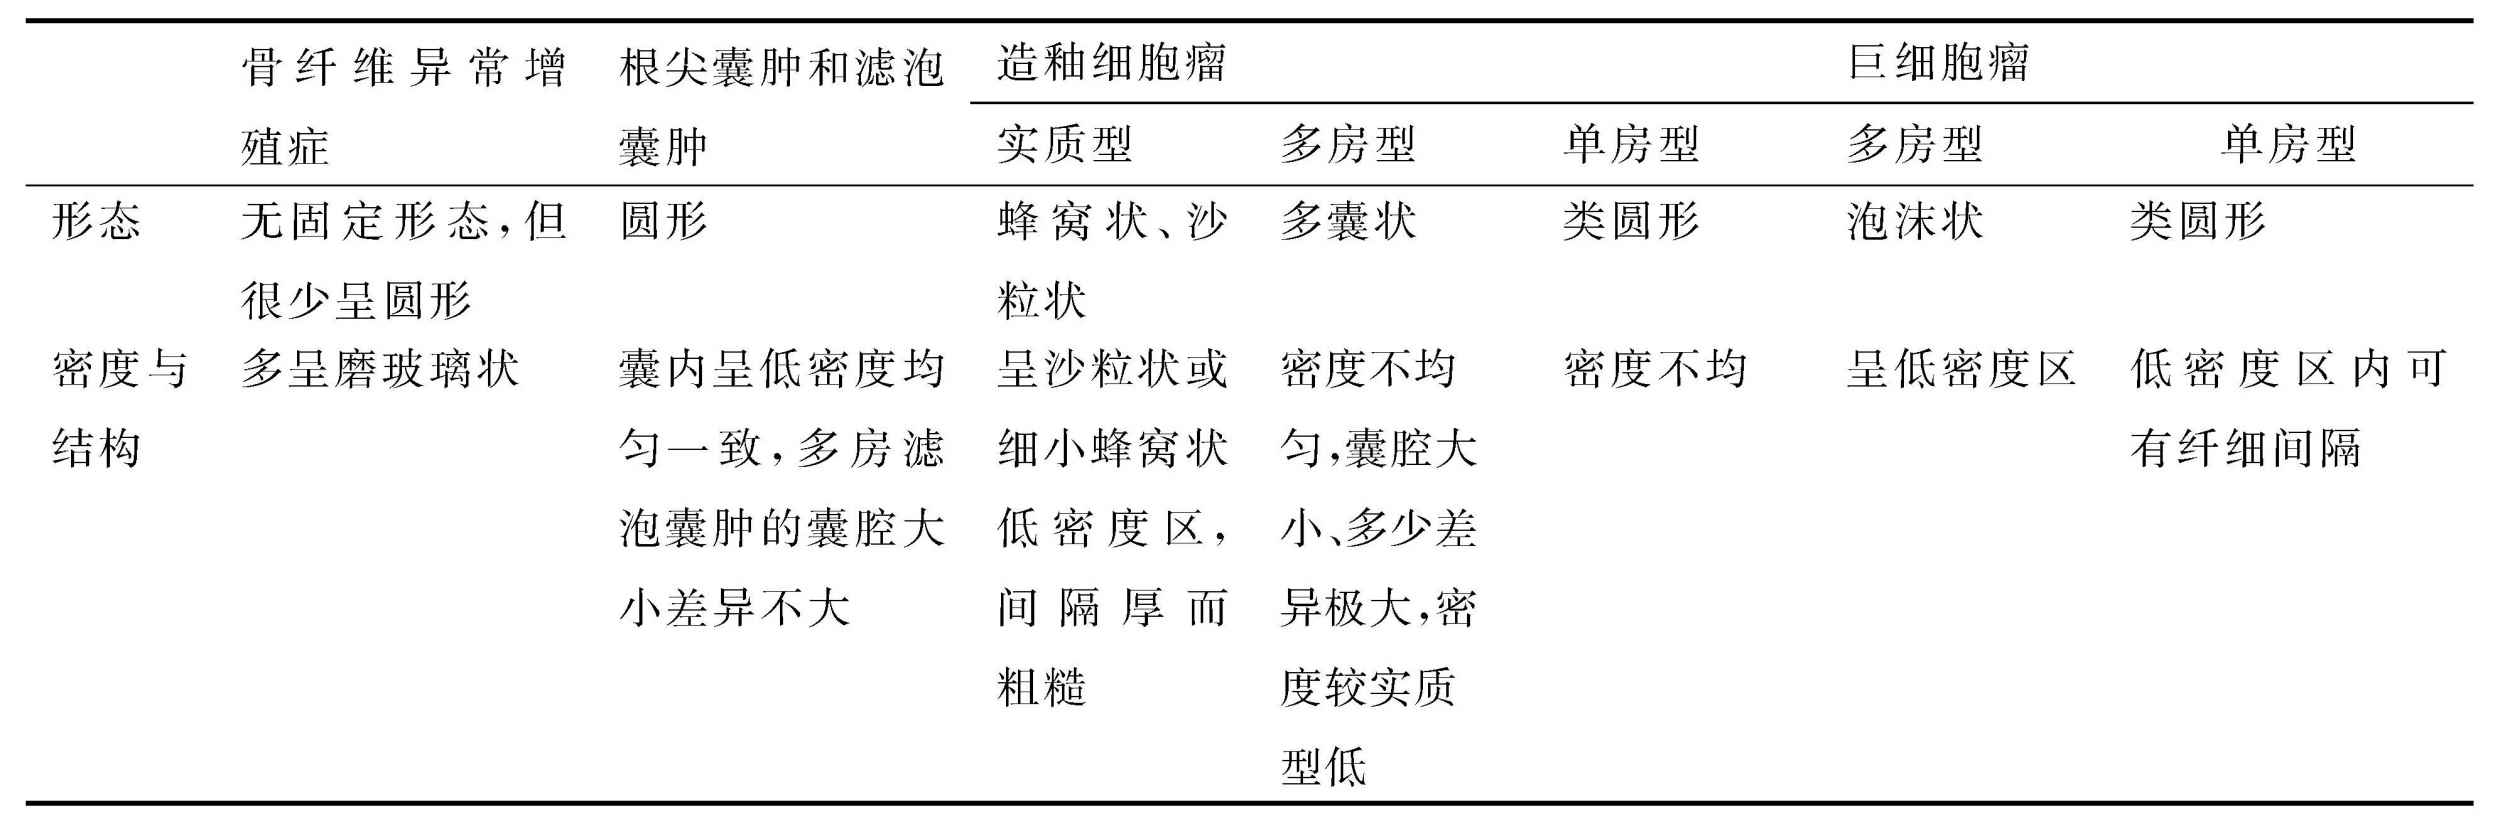
\includegraphics[width=\textwidth,height=\textheight,keepaspectratio]{./images/Image00159.jpg}\\
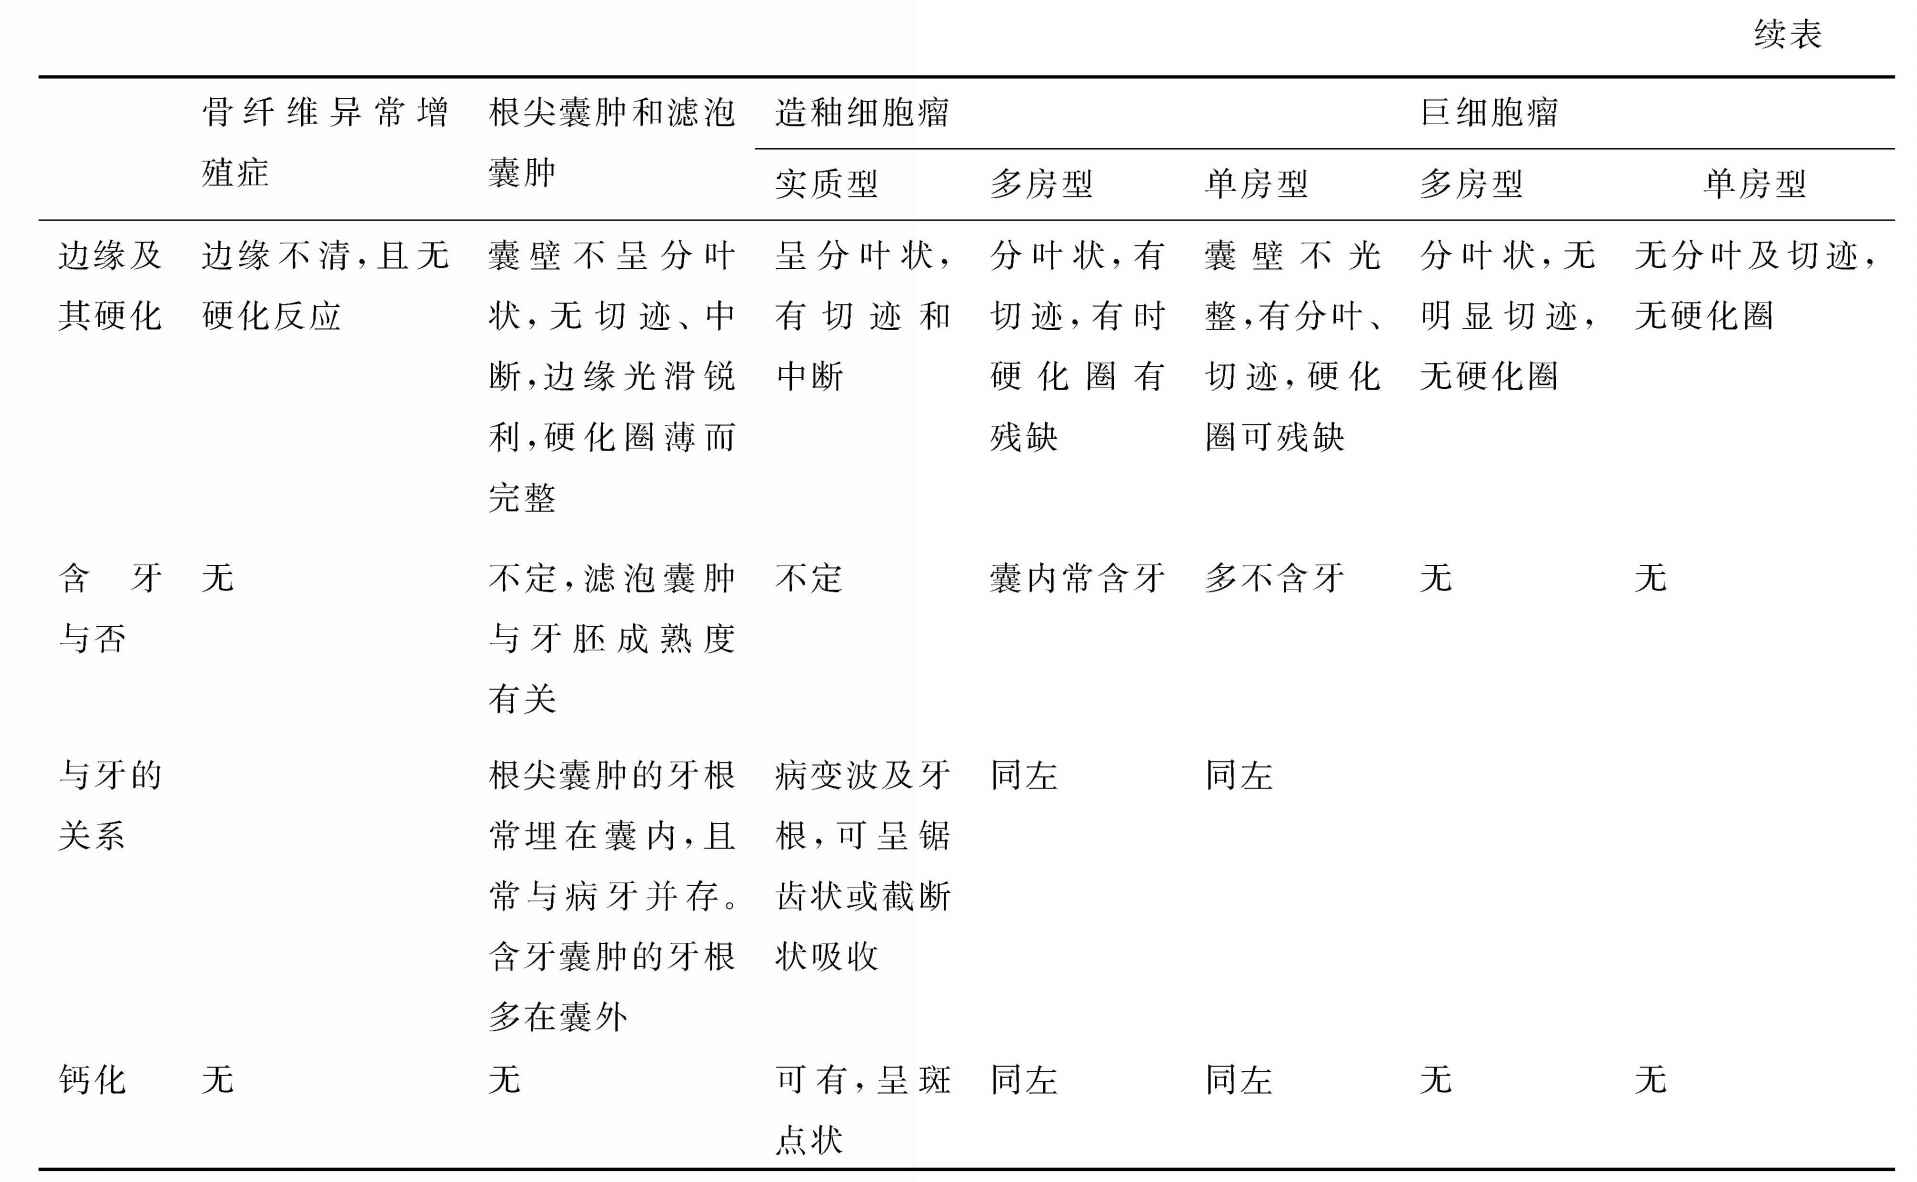
\includegraphics[width=\textwidth,height=\textheight,keepaspectratio]{./images/Image00160.jpg}
\end{longtable}



\subsection{牙源性腺样瘤}

本病以往被认为是造釉细胞瘤的一型而有腺样造釉细胞瘤之称,但临床和病理形态上均有其特点。1971年,WHO已将此瘤列为颌骨的一种独立肿瘤。

\textbf{【病理】}
肿瘤多较小,直径一般<3cm,巨检包膜完整,多呈囊状,囊壁较厚,囊内可含牙。镜下肿瘤上皮可有不同的形态结构,其内常见小钙化灶。

\textbf{【临床表现】}
该病女性多于男性,多见于青少年(20岁左右)。上颌比下颌多,以单尖牙区最多见。一般无症状,或仅有膨胀感。常见有未萌牙。肿瘤属良性,刮除后不易复发。

\textbf{【影像学表现】}
以单房多见,边缘无硬化。骨皮质膨胀不显著,无侵蚀,无皮质破坏征象。肿瘤内含有未萌出的牙,其中以单尖牙最多见,其次为第一双尖牙及侧切牙。乳牙常滞留。瘤体内可见多数钙化小点呈粟粒状。

\subsection{牙瘤}

本病是由牙胚组织异常发育增生而形成的,属成牙组织发育畸形,而非真性肿瘤。

\textbf{【病理】}
肿瘤内含有牙釉质、牙骨质、牙本质和牙髓。组织学通常分为3型:①混合型牙瘤:为各种牙组织混合而成,排列紊乱,形态不一。一般为圆形或卵圆形钙化团块,周围被以纤维膜。②组合型牙瘤:由大小不等、形成较好、大小不定的牙齿组合而成。牙齿数目不等,由数个至数百个。③囊性牙瘤:类似含牙囊肿。不同数目的小齿或牙质小碎片包括在囊腔内。

\textbf{【临床表现】}
多见儿童和青年。一般无自觉症状,可见颌骨膨胀。手术切除不复发。

\textbf{【影像学表现】}
①混合型:多位于磨牙区。可见颌骨骨质膨胀和一团相当于牙齿硬组织密度的影像,分不出牙齿的形态。团块与正常骨之间有一条清晰的低密度区为牙瘤的包膜。②组合型:多位于前牙区。表现为大小不等、形态不定、类似发育不全的小牙堆积在一起。③囊性牙瘤:见囊样低密度区中含有高密度之小齿或高密度碎骨块样病灶。

\subsection{假性牙骨质瘤}

本病亦称为牙骨质结构不良,但不属于真正的肿瘤。

\textbf{【病因病理】}
病因不明,可能与咬颌创伤有关,是较常见的根周病变。多数认为是牙骨质发生的,但亦有人认为来自根尖部的骨组织。①早期:又称为溶骨期。患牙根周围的骨质被纤维组织所代替。②中期:在根尖周围增生的纤维结缔组织中,有部分牙骨质或球形牙骨质小体形成。③后期:又称成熟期。病变由球形牙骨质小体、增生较大的牙骨质团块及钙化似网状的骨组织结合构成。

\textbf{【临床表现】}
多发生于中年女性,平均年龄40岁左右。本病一般无自觉症状,好发于下颌切牙区,常有牙松动。少数出现根尖周炎的表现。

\textbf{【影像学表现】} 病理改变分为3期,故影像学表现分为3型。

1.早期:又称为溶骨期。表现为囊状低密度区,颇似根尖肉芽肿和根尖囊肿。单凭影像学难以做出诊断,但患牙仍有活力,根周膜完整。

2.中期:表现在骨质破坏区中心先后出现点状或小团状钙化影,病变外围仍呈环形低密度区。

3.后期:又称成熟期。表现为在根尖周围区呈界限清楚、密度较高的钙化团块影,其周边有一薄层线状低密度环。牙周膜及骨硬板清楚。

\textbf{【鉴别诊断】}
本病应与真性牙骨质瘤即良性牙骨质母细胞瘤鉴别。后者多发生于25岁以下男性,以下颌第一磨牙的根尖周围多见。影像学不易区别,以病理诊断为准。

\subsection{真性牙骨质瘤}

本病又称为良性牙骨质母细胞瘤、良性成牙骨质细胞瘤。

\textbf{【病理】}
肿瘤大部分为钙化组织,内含少量类似于牙骨质的细胞,其周缘有结缔组织包膜。

\textbf{【临床表现】}
该病多发生于25岁以下男性,以下颌第一磨牙的根尖周围多见。一般无自觉症状,可引起颌骨膨胀和疼痛。

\textbf{【影像学表现】}
表现为团块状密度增高区,周围有低密度包膜。病变附于牙根处,可伴牙根吸收或牙根与肿瘤融合。

\subsection{牙源性钙化囊肿}

本病是一种少见的牙源性病变。最近研究发现兼有囊肿和实质性肿瘤的许多特征。

\textbf{【病理】}
巨检为囊性或实质性两种。有大量角化物或钙化物,有完整的包膜。部分病变内有发育不良的牙本质和牙瘤成分。本病有骨内型和骨外型之分。

\textbf{【临床表现】}
可发生于任何年龄,但有20岁和60~70岁两个发病高峰期。性别无差异。多无症状。手术摘除不易复发。

\textbf{【影像学表现】}
上、下颌发病率相近,常发生于颌骨磨牙及双尖牙区。颌骨内单房或多房囊状低密度区,形态不规则,界限清楚,瘤体内可含牙并可见大小不等的钙化点、钙化灶或不规则钙化团。病变累及的牙根可有吸收,邻牙可有移位。

影像学难与造釉细胞瘤、牙源性腺样瘤、囊性牙瘤等相鉴别。

\subsection{牙源性钙化上皮瘤}

本病又名Pindborg瘤,较少见。

\textbf{【病理】}
巨检为实质性,浸润骨组织。有的无包膜或包膜不完整。瘤体内上皮细胞可有淀粉样变,这种变性细胞内或其周围常发生钙化,钙化呈同心圆沉积。肿瘤生长缓慢,虽属良性,但有局部侵蚀性,手术不彻底易复发。

\textbf{【临床表现】}
多见于20~60岁,其性别无差异。多无自觉症状,局部颌骨膨大,患区有未萌牙或埋伏牙。

\textbf{【影像学表现】}
下颌比上颌多见,最常发生的部位是磨牙和双尖牙区,尤以前者更多见。表现为颌骨不规则骨质破坏,可呈单房、多房或蜂窝状,其中含有大小不等的钙化团块。常有埋伏牙。可使颌骨膨大,骨皮质破坏。发生于上颌骨者,可见上颌窦壁被破坏。

\subsection{牙源性纤维瘤}

本病少见。源自中胚层,发生于牙乳头或牙囊的间质细胞,在成人源自牙周膜。

\textbf{【病理】}
肿瘤由大量较成熟的纤维结缔组织组成,但多少有成骨活动。肿瘤内偶见牙骨质小体形成。此瘤为良性,可恶变为肉瘤。

\textbf{【临床表现】}
发病年龄广泛,常见于青少年,无性别差异。多无自觉症状。切除后不易复发。

\textbf{【影像学表现】}
下颌多于上颌,生长缓慢。常为多房,分隔少,隔较直且欠清晰锐利,房室多呈方形或多边形;单房者无切迹。瘤内密度不均,可有不规则高密度灶。颌骨多膨胀。可伴有牙根吸收、邻牙移位或缺失,瘤内可含牙。

\subsection{牙源性黏液瘤}

本病少见,多认为属良性肿瘤,少数认为属低度恶性肿瘤。肿瘤起源于中胚层结构,亦可为牙源性纤维瘤退变而来。

\textbf{【病理】}
切面呈胶冻状,内含黏液及少量牙源性上皮条索。肿瘤多无包膜,偶尔有不完整的包膜。镜下见在梭形或星形瘤细胞之间有大量黏液样物。一般生长缓慢,呈局部浸润性生长。

\textbf{【临床表现】}
主要见于青壮年人,性别无明显差异。病变生长缓慢,可使邻牙移位,术后易复发。

\textbf{【影像学表现】}
下颌多于上颌,多位于下颌双尖牙或磨牙区,可缺牙或含埋伏牙。肿瘤呈囊状膨胀性生长,与周围骨质界限不清。低密度区内常有垂直排列的小梁状钙化或骨性分隔,似线网状或“火焰状”。亦可呈多囊状或蜂窝状低密度区。肿瘤大者可穿破皮质形成软组织肿块,残存的垂直钙化小梁呈放射状骨针,勿误为恶性肿瘤。

\subsection{化牙骨质纤维瘤}

本病又称牙骨质纤维瘤,是颌骨少见的中心性良性肿瘤。

\textbf{【病理】}
肿瘤由胶原纤维、成纤维细胞、成牙骨质细胞组成。在纤维组织内有数量不等的牙骨质小体。肿瘤生长缓慢,术后较少复发。

\textbf{【临床表现】}
可发生于任何年龄,常见于中年人,女性略多。生长缓慢,可使颌骨膨大变形、邻近牙移位。

\textbf{【影像学表现】}
多位于下颌双尖牙和磨牙区。本病呈单囊状或多囊状骨质破坏,有的呈皂泡状,破坏区边缘整齐。颌骨骨质膨胀,无断裂。肿瘤内可见弥散性的斑片状高密度影,有时可见圆形高密度牙骨质小体。可含牙,牙根居病变之中,一般无侵蚀。相关牙可移位。

\subsection{颌骨骨化性纤维瘤}

本病又称骨性纤维瘤、成骨性纤维瘤及纤维骨瘤等。有人根据其成分不同而分别用其名称,如病变以骨组织为主称为纤维骨瘤,若病变以纤维成分为主则称为骨化性纤维瘤。

\textbf{【病理】}
肿瘤来源于颌骨内成骨性结缔组织。瘤组织由纤维组织和骨组织组成,且两种成分比例可各不相同,故各个肿瘤的组织学表现亦不一致。肿瘤有包膜、界限清楚,这是本病区别于骨纤维异常增殖症的特征之一。

\textbf{【临床表现】}
本病常见于青少年,以女性多见。生长缓慢,早期无自觉症状,逐渐使颌骨膨大而就诊。

\textbf{【影像学表现】}
此病多发于颌骨,尤以下颌骨多见。通常分为3型:①硬化型:病变区骨组织多于纤维组织。表现为圆形或椭圆形高密度区,呈密度不均的斑片状,甚至呈一致密骨块。边缘整齐清楚,但亦可呈分叶状。邻近骨组织可受压。②囊型:病变区纤维组织多于骨组织。表现为圆形、椭圆形或不规则形低密度区,呈单房或多房膨胀性生长,边缘清晰,与正常骨组织界限明显。低密度区内有数量不等的高密度骨化或钙化影。周围骨组织轻度硬化。③混合型:兼有以上两型的改变。

\textbf{【鉴别诊断】}

1.骨纤维异常增殖症:是以骨内纤维组织异常增生并有编织骨形成为特征的瘤样病变或骨质生长发育障碍。①因骨纤维异常增殖症无包膜,故边界模糊不清。病变范围较大,呈弥漫膨胀性,邻近牙一般无吸收。②骨纤维异常增殖症发生于上颌骨者上颌窦明显缩小或闭塞;位于下颌骨者,下颌骨常呈磨玻璃样,界限不清晰。③病变的生长方式,在下颌骨者沿长轴生长;在上颌骨者沿上颌窦骨壁弥漫生长,保持上颌骨凹陷外形。

而骨化性纤维瘤系肿瘤病变,有包膜、界限清,病变范围局限,近圆形膨胀性生长。

2.造釉细胞瘤:好发于下颌骨磨牙区。肿瘤边缘呈分叶状,大小囊悬殊大,有切迹和中断,密度不均,易向牙槽突突破形成软组织肿块或根间浸润。瘤区牙根吸收较明显。这些可与骨化性纤维瘤相鉴别。

\subsection{颌骨巨细胞瘤}

本病又称为破骨细胞瘤,不常见。

\textbf{【病理】}
有人分为中央型及周围型两型。中央型者多位于下颌联合及前磨牙区。发生于上颌骨者多位于尖牙窝。周围型者多位于下颌齿槽突部,常突入口腔成为巨细胞龈瘤。镜下主要由多核巨细胞和间质细胞组成。

\textbf{【临床表现】}
本病多发生于青壮年,以20~40岁多见。性别无差异。常表现为颌骨膨胀、面部畸形,可伴间歇隐痛,邻近牙齿松动。

\textbf{【影像学表现】}
呈单囊或多囊状溶骨性破坏。单囊状少见,大小不一,边缘欠清楚,瘤内有少量不规则条纹状高密度影。多囊状多见,呈多个小或大小不均的囊状低密度区,边缘清楚,膨胀性生长,骨皮质变薄,很少穿破皮层。病灶周围无硬化带。增强扫描可有中度强化。

\subsection{颌骨血管瘤}

颌骨血管瘤少见,下颌多于上颌,以中央型多见。

\textbf{【临床表现】}
好发于20岁左右。表现为颌骨缓慢生长的无痛性肿块。患区牙齿反复出血、牙齿松动,拔牙则产生严重出血。

\textbf{【影像学表现】}

1.中央型:病变好发于下颌骨体部,沿水平方向膨胀性扩展。病变早期骨小梁疏松,呈水平方向吸收消失。随着病变发展,形成粗网状、蜂窝状或肥皂泡状骨质破坏,也可形成较大的囊状破坏,边界模糊。可出现牙周硬板吸收消失,牙根移位或吸收。下颌管扩张下移、颏孔增大,是下颌骨中心性血管瘤的特征性表现。少数病例骨小梁呈放射状排列。少数病例伴发颌周围软组织肿胀并可见静脉石。CT增强扫描病灶明显强化。

2.周围型:起源于骨膜,很少见。骨皮质局限吸收,可侵及松质骨,向外生长形成密度不均的软组织肿块。CT增强扫描病灶明显强化。

\subsection{颌骨恶性肿瘤}

颌骨恶性肿瘤分为3大类:①原发性恶性骨肿瘤:最常见者有骨肉瘤、纤维肉瘤、软骨肉瘤、骨髓瘤、尤文肉瘤、恶性纤维组细胞瘤及颌骨中央性癌等。②继发性恶性骨肿瘤:为附近组织恶性肿瘤扩延至颌骨所致。牙龈癌以及其他软组织恶性肿瘤均可侵及邻近颌骨组织,其中以龈癌为最多,其次为上颌窦、腭、口底、颊、舌等部位的恶性肿瘤。③颌骨转移性恶性肿瘤:临床不常见。为其他器官的原发恶性肿瘤转移至颌骨。以上3类中以继发性颌骨恶性肿瘤最多见。

\textbf{【影像学表现】}
其共性表现为溶骨性不规则骨质破坏伴软组织肿块。成骨肉瘤有不规则瘤骨、骨膜反应;软骨肉瘤有不规则钙化表现;尤文氏肉瘤病变周缘有新骨增生(部分呈放射状骨针)、多伴有葱皮状骨膜反应;转移性肿瘤一般有溶骨、成骨和混合性3类。CT增强扫描轻度或无明显强化。

牙龈癌可见牙龈肿胀,局部形成软组织肿块。早期邻近颌骨牙槽突有界限不清的骨质吸收;进一步发展,局部出现扇形骨质破坏区,口宽底窄,分化好者边缘整齐,分化差者边缘呈蚕食状。同时可发现局部淋巴结转移。

\subsection{颌骨中央癌}

\textbf{【病因病理】}
可能起源于胚胎时期面突融合处的上皮残余或牙源性上皮残余。为全身骨骼中惟一能发生原发癌的骨骼。通常为鳞癌,亦可为腺癌。因肿瘤自骨髓腔向骨皮质浸润,可在邻近软组织出现肿块,牙齿可松动、脱落。

\textbf{【临床表现】}
成年人多见,男多于女。多见于下颌磨牙区。下唇麻木和神经疼痛为侵犯神经的早期症状,累及牙时可有酸痛,患区颌骨可轻度膨隆。

\textbf{【影像学表现】}
颌骨内虫蚀样溶骨性骨质破坏。下颌者早期侵犯下颌管。病变向牙槽骨方向扩展时,可使牙周组织破坏消融,牙齿浮于软组织中,以致脱落。病变继续进展则侵犯骨皮质。病变界限不清,无骨膜反应及新骨形成,无钙化。晚期可并发病理骨折,浸润软组织及皮肤。侵犯颌外软组织则难以判断原发部位。

\textbf{【鉴别诊断】}
中央性颌骨骨髓炎有炎症病史。影像学可见骨质破坏以病源牙为中心,逐渐移行于正常骨组织。有死骨及骨质增生等可资鉴别。

\section{涎腺疾病}

\subsection{腮腺炎症}

腮腺炎临床较为多见。

\textbf{【病因和分类】}
其分类方法有多种:①按病原体分为:化脓性、特异性(如结核)和病毒性,以化脓性最多见。②按病程分为:急性和慢性,慢性多于急性。急性多见于儿童,成人则以慢性炎症多见。慢性化脓性腮腺炎多由结石、异物、导管狭窄、导管开口位置异常等原因所致。③国外有学者将腮腺炎性病变分为阻塞性、非阻塞性、肉芽肿性及舍格林综合征。④国内有学者将慢性化脓性炎症分为儿童复发性、成人复发性、慢性阻塞性及腮腺内非特异性淋巴结炎,其中腮腺内非特异性淋巴结炎为假性腮腺炎。

\textbf{【病理】}
大部分腮腺炎腺体体积增大,急性期尤为明显,至慢性期腮腺可持续性增大,亦可腺体萎缩、纤维化、体积缩小。慢性炎症导致腺体体积增大与其病理过程有关。当炎症转入慢性期导管周围炎性反应增强,结缔组织纤维化,大量淋巴细胞、组织细胞及巨噬细胞浸润,近腺体段导管明显扩张,故腮腺体积持续增大,密度增高。

\textbf{【CT表现】}
可概括为3种类型:①双侧或单侧腮腺弥漫性增大,密度均匀增高,与周围结构分界清楚。增强后轻度强化。②单侧腮腺弥漫性增大,密度多不均匀,边缘模糊,与咬肌分界欠清晰。增强后不均匀强化。③单侧腮腺内局限性高密度影,密度较均匀,边缘模糊。增强后轻度强化,界限稍清晰。④腮腺慢性炎症伴有淋巴结反应性增生,表现为密度均匀的结节状。病灶内局限性结节一般较小,直径多<1.5cm,且为多个,有别于良性肿瘤。

此外,如肿胀区内出现液平面,常提示为脓肿形成。并应注意有否结石,结石好发于颌下腺,其次为腮腺,以导管内结石多见,它是阻塞性化脓性炎症的原因之一。

\textbf{【鉴别诊断】}

1.腮腺恶性肿瘤:炎症可双侧,亦可单侧;而肿瘤多为单侧发病,极少双侧,故双侧弥漫性炎症较易诊断。单侧腮腺弥漫性炎症如合并导管阻塞、扩张、积液,且与病灶周围结构界限不清,则不易与恶性肿瘤相鉴别(如恶性淋巴瘤可呈弥漫性肿块)。但炎症扩张的导管往往沿腮腺导管分布方向走行,如多处导管扩张、边界清晰、呈放射状分布,与恶性肿瘤不均匀坏死有明显不同,诊断不难。如单发导管扩张致条状低密度,则诊断较为困难,必须结合临床。增强扫描有助于诊断。

2.腮腺腺淋巴瘤:可双侧发病;腺淋巴瘤为良性病变,易囊变;早期迅速强化、无延迟强化。与慢性炎症性囊样病变相比囊变范围较小,边界模糊。

3.腮腺血管瘤:多为单侧弥漫性病变。一般密度较均匀,边界模糊或清晰。增强后强化明显且持续时间长。

4.腮腺混合瘤:单侧腮腺局限性炎症,部分病例因病灶密度较高、均匀,增强后轻度强化,不易与腮腺混合瘤鉴别。但混合瘤多为类圆形结节状软组织肿块,边缘锐利、光滑,与正常低密度的腺体分界清楚。常为中度或中度以上强化,亦可呈均一或环形强化。国外报道于120秒有延迟强化。当肿瘤有囊变时,平扫和增强扫描均呈规则或不规则液性密度区,但确诊有赖于活检。

5.腮腺囊性病变:腮腺炎症或结石导致腮腺导管阻塞、扩张、积液形成潴留囊肿时,应与囊性病变相区别。囊性病变有单纯囊肿和囊性肿瘤(如腺淋巴瘤囊变、咽旁间隙的神经源性肿瘤囊性变),如病灶与腮腺界限不清时,难与腮腺炎症鉴别。但单纯囊肿和囊性肿瘤的囊多较大,壁清晰,周边界限多清晰,而炎症所致导管扩张多表现为条状低密度影,张力不高,周边结构模糊,可资鉴别。

\subsection{涎腺结核}

涎腺结核一般多发生于腮腺,常为单侧性;颌下腺次之;舌下腺和小涎腺很少见。

\textbf{【病因病理】}
涎腺(尤其是腮腺)的腺体内和腺体外有丰富的淋巴组织,包括数目众多的淋巴结和淋巴管网,故涎腺结核的感染途径大多经淋巴系统,首先侵犯淋巴结而后波及涎腺。也可为管源性和血源性。病理改变与一般淋巴结核相仿,主要是炎症和干酪坏死。

\textbf{【临床表现】}
约1/3发生于20~30岁。可分为慢性包块型和急性炎症型。主要表现为腺体肿胀和略有疼痛,肿大的涎腺质地稍硬,如形成冷脓肿后质地变软。冷脓肿与导管相通后,脓液可由导管口流出。

\textbf{【影像学表现】}
①病灶局限于淋巴结内,使淋巴结增大,呈软组织样密度灶,腺体造影见导管受压推移,似涎腺良性肿瘤所见。②如病变进展,组织分解形成空洞,波及涎腺实质,则形成界限不清之软组织样密度增高区,腺体造影见造影剂外溢呈团块状,似涎腺恶性肿瘤所见。管源性者亦可直接侵及涎腺,呈上述表现。③如向皮肤破溃形成瘘管,需腺体造影观察。

总之,无论就临床还是影像学而言,涎腺结核不易与涎腺良、恶性肿瘤相鉴别。

\subsection{舍格林(Sjogren)综合征}

本病命名颇为混乱。1888年,Mikulicz首先报告双侧腮腺、泪腺肿大病例,此后此类病以米枯力滋病命名。1933年,Sjogren报告干燥性角膜炎、多发性关节炎、腮腺肿大并存的病例。目前认为口干、眼干及结缔组织病这3种中有两种表现存在,足以诊断舍格林(Sjogren)综合征,即干燥综合征。1952年,Good-Wine将米枯力滋病的病理变化称为良性淋巴上皮病变。1953年,Morgan及Castlemen根据以上两者均有涎腺内淋巴组织增生性病变,而认为二者是同一疾病过程,米枯力滋病是舍格林综合征的一种变异。目前认为两者之间的确切关系尚需进一步研究,仍应考虑为两种不同的疾病。“良性淋巴上皮病变”并非完全良性,有的可有恶变。

\textbf{【病因病理】}
舍格林(Sjogren)综合征是一种以外分泌腺损害为主的自体免疫性疾病。经临床检验证实:有口干和眼干者为原发性;有口干和(或)眼干伴有结缔组织疾病(常见的有类风湿关节炎、SLE、硬皮病和多发性肌炎等)者为继发性舍格林综合征。原发性和继发性病理表现基本相同,镜下主要表现是淋巴细胞和组织细胞增生浸润。

\textbf{【临床表现】}
多见于中老年女性,男女之比约1∶10。可单侧或双侧腮腺或(和)颌下腺肿大,舌下腺及其小涎腺亦可肿大,可继发感染,有的伴泪腺肿大,有口干、眼干、类风湿关节炎或其他结缔组织疾病症状及相应实验室检查改变。

\textbf{【影像学表现】}
①腺体形态正常,排空功能差:需腮腺造影观察排空情况。CT可见腮腺肿大,密度普遍性增高,其间有小囊状透亮区。CT腺体造影可见肿大腺体内不规则充盈缺损,结构有破坏。②涎腺导管扩张:主导管多无改变,其他导管有的呈羽毛状、花边状、葱皮状变形。腺体内导管分支异常细、稀少或不显影。末梢导管有轻重不同的扩张。CT腺体造影表现为有散在点状造影剂存留。③向心性萎缩:表现为体积缩小。腺体造影仅见主导管及某些叶间导管显影,周缘腺体组织不显影。④肿瘤样改变:有的似良性肿瘤,有的似低度恶性肿瘤或恶性肿瘤,这是由于局部被侵蚀的小叶融合在一起形成包块所致。有的确实已经恶性变。

\textbf{【鉴别诊断】}

1.涎腺肿瘤:如舍格林综合征临床及CT有占位表现,造影又发现肿瘤样所见,则难以与肿瘤区别。但如造影同时伴有末梢导管扩张,CT及X线发现其他涎腺亦有异常者,结合临床有助于与肿瘤鉴别。

2.慢性化脓性腮腺炎:临床可见涎液及较多的脓液。不像舍格林综合征一般无脓,即使继发感染脓也很少。腺体造影慢性化脓性腮腺炎主导管改变呈腊肠样,但无边缘羽毛状、花边状、葱皮状变形以及腺体内充盈缺损。有时早期难以区别。

3.涎腺良性肥大:常见于腮腺,而颌下腺少见。病因不明,常与内分泌失调(如妇女绝经期、甲状腺功能低下者、糖尿病患者等)有关。涎腺形态多正常,体积明显增大;可伴有导管轻度扩张、排空功能差,但程度不及舍格林综合征。结合病史及化验检查可协助诊断。

\subsection{恶性肿瘤(概述)}

涎腺肿瘤颇为常见,多数来源于腺组织,少数来自间叶组织,种类不少(见表\ref{tab7-3})。其中混合瘤占良性肿瘤的90%以上,好发于腮腺;恶性肿瘤好发于腮腺及颌下腺。

\begin{table}[htbp]
\centering
\caption{涎腺肿瘤的分类}
\label{tab7-3}
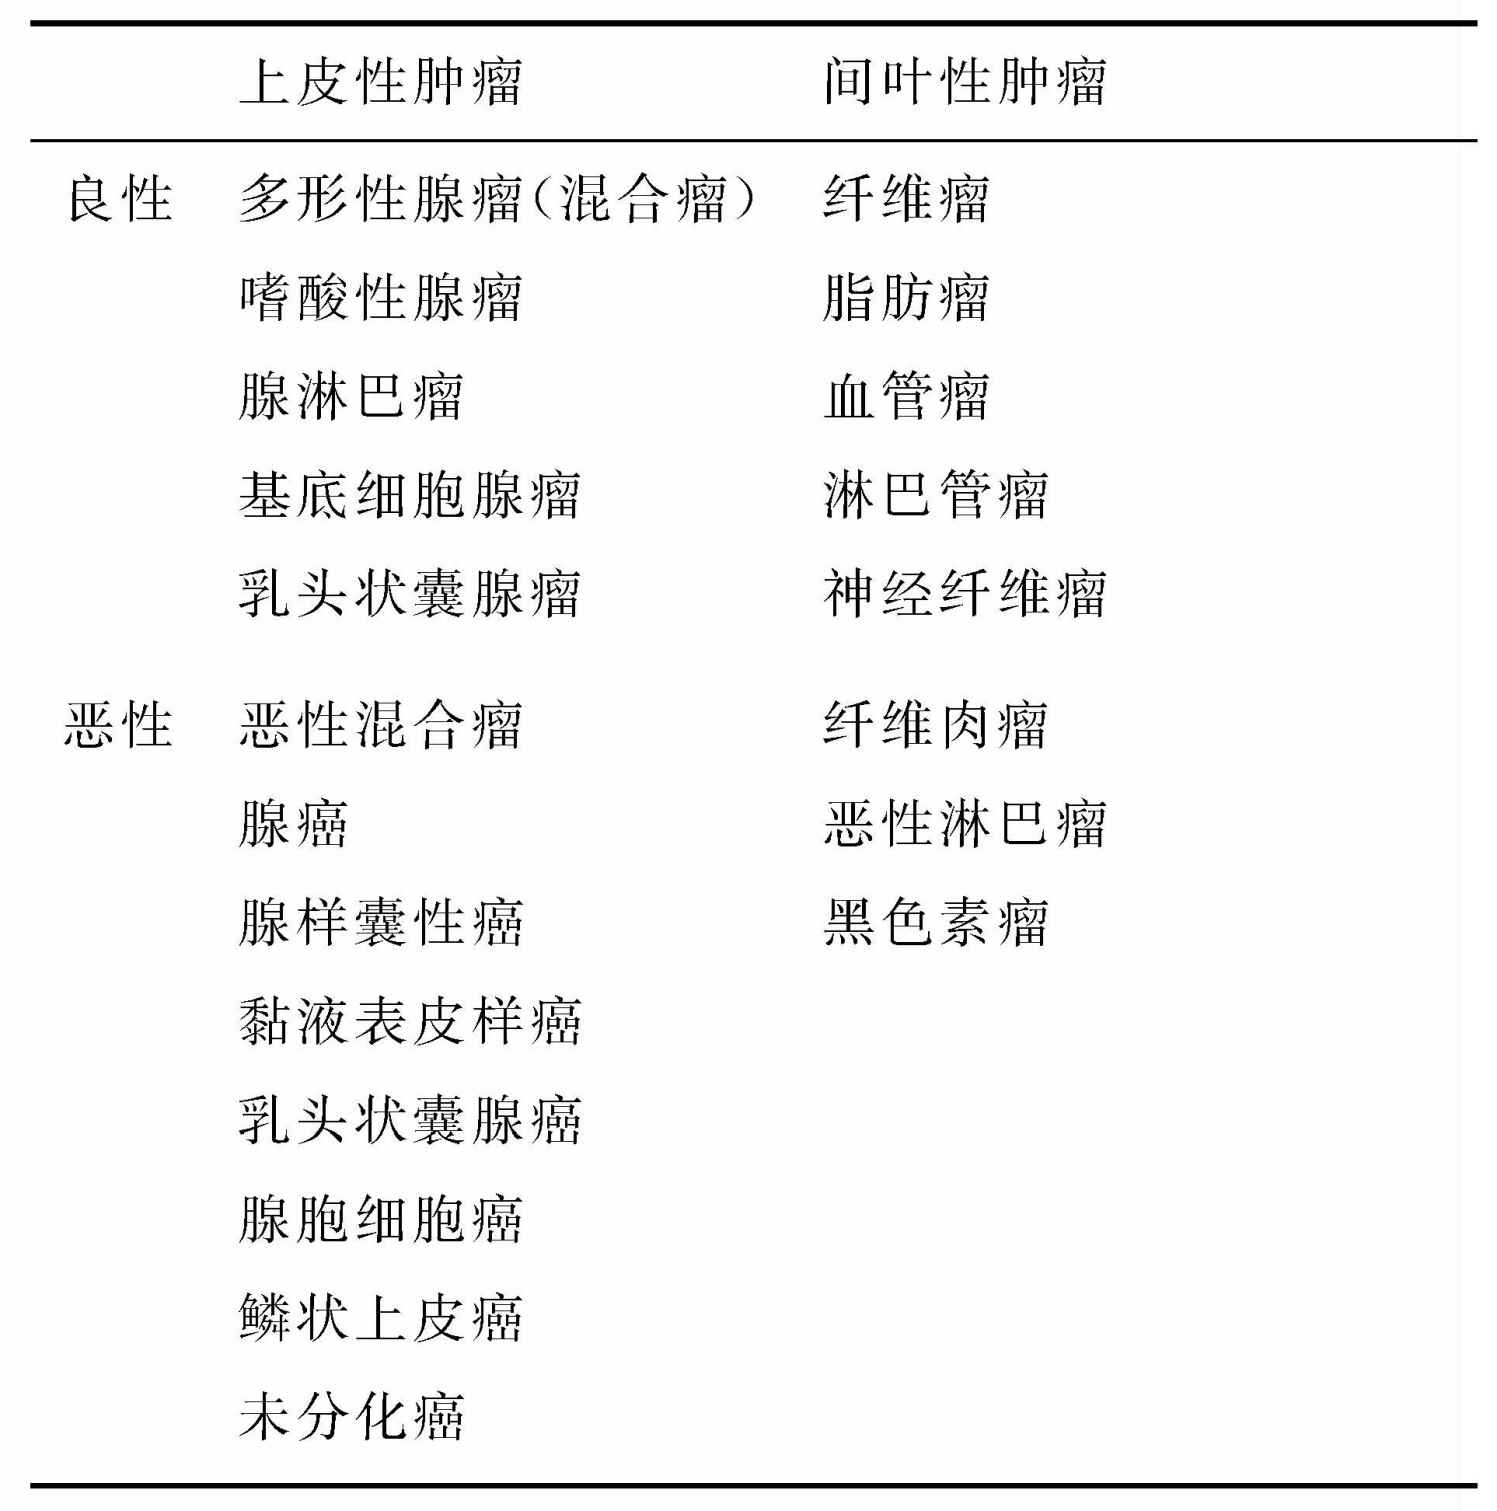
\includegraphics[width=\textwidth,height=\textheight,keepaspectratio]{./images/Image00161.jpg}
\end{table}

\textbf{【CT表现】}

1.良性肿瘤:①多呈圆形或类圆形,界限清楚,边缘光滑,密度均匀,CT值多在30~45Hu;②腺体造影后CT表现为边缘清楚的低密度区;③静脉增强扫描时,肿瘤均匀性强化,CT值多在62Hu以上;④良性肿瘤的内部可见低密度,多由于其内的黏液变性、囊变引起,可多发,但较少融合;⑤脂肪瘤呈典型界限清晰的脂肪密度,CT值-100Hu左右;⑥血管瘤和血管淋巴瘤好发于婴幼儿,海绵状血管瘤如显示静脉石,是其特征性表现。

2.恶性肿瘤:①肿瘤形态不规则,界限不甚清楚或完全不清;②内部密度不均,一般来说恶性肿瘤的中央低密度区较大、融合,为坏死出血所致;③皮下脂肪层及腮腺咬肌筋膜界面消失;④肿瘤侵及皮肤、咬肌、胸锁乳突肌及翼内肌时,可模糊不清,有的可见颞骨岩部或乳突骨质破坏;⑤恶性肿瘤血供丰富,常有明显强化,肿瘤与邻近肌肉密度差50Hu左右时应警惕恶性可能。总之,边缘不规则,界限不清,明显强化,内部密度不均,以及颌部淋巴结肿大为原发恶性肿瘤的特点。面神经受累症状为腮腺恶性肿瘤的临床特点。

良、恶性肿瘤除上述典型表现外,尚有部分肿瘤表现为界限清楚,但边缘不规则,呈结节状,内部均匀或不甚均匀,术后多证实为混合瘤或低度恶性肿瘤。

\subsection{腮腺肿瘤}

腮腺肿瘤占全部唾液腺肿瘤的70%~80%,且腮腺肿瘤中80%是良性肿瘤,而颌下腺肿瘤约占20%,且50%以上是恶性肿瘤。良性者不像其他部位的良性肿瘤,具有完全的良性性质,而是带有一种不稳定的倾向。而恶性肿瘤与其他部位者相比,恶性程度较低,术后生存可长达20年以上。但无论是良性或恶性腮腺肿瘤,其生长方式和大体形态的CT表现都不能做出组织学诊断。

\textbf{【CT表现】}
国外有学者把腮腺肿瘤的CT表现分为3类:①界限清楚的圆形肿瘤;②界限清楚的分叶状或不规则肿瘤;③界限不清的弥漫性不规则肿瘤。这3种表现基本反映了3类肿瘤的性质,即良性肿瘤、具有侵袭性的良性肿瘤或低度恶性肿瘤、侵袭性较强的恶性肿瘤。但恶性肿瘤亦可界限清楚,边缘光整;生长迅速的良性肿瘤亦可边缘模糊。

\textbf{【鉴别诊断】}
腮腺外肿块常见的有脓肿、增大淋巴结、淋巴瘤或颈动脉间隙内的血管瘤、神经源性肿瘤或腮裂囊肿等。

腮腺内、外肿瘤的鉴别依据是:①腮腺外肿瘤与正常腮腺组织间常有一脂肪线分界,是诊断腮腺外肿瘤的惟一可靠依据。②CT腮腺造影示充盈的腺体与腺外肿瘤密度对比明显,即使无脂肪线,亦可见与腺外肿瘤的界限。后者致正常的腮腺受压移位,有时边缘可见弧形压迹或缺损。③腮腺深叶肿瘤常使咽旁间隙内的脂肪向前、内移位,下颌茎突间隙增宽;而咽旁间隙茎突前区肿瘤多使咽旁间隙内的脂肪外移,下颌茎突间距变窄;而咽旁间隙茎突后区肿瘤将咽旁间隙向外推移,将茎突向外、向前推移。

\subsection{腮腺混合瘤}

本病亦称多形性腺瘤。是腮腺最常见的肿瘤,占腮腺肿瘤的60%~70%,其中90%为良性,10%为恶性。

\textbf{【病理】}
因肿瘤由腺上皮和肌上皮细胞(其间散布各种间质)组成,故称为混合瘤。肿瘤内基质或黏液样物质的含量变化范围很大,但很少有钙化。约34%的肿瘤可呈不均匀的膨胀性生长而形成多结节状。包膜可完整或不完整,厚薄不一。恶性混合瘤可以是:①良性混合瘤合并癌,最为常见;②癌及肉瘤并存;③良性多形性腺瘤有远处转移,即恶变。良性多形性腺瘤存在的时间越长,恶变率越高,如不及时切除约25%会合并癌。

\textbf{【临床表现】}
常见于30~50岁,男女发病相近。早期多无症状,多在发病后数年就诊。多表现为无痛性肿块,位于耳垂下或后方,有时也可位于耳屏前。肿块与皮肤无粘连。约10%位于颌骨后腺体而表现为口咽侧壁膨隆,甚至张口受限。恶性者发病年龄偏大(40岁左右),肿块增大快,活动度差,伴有局部疼痛,多有面神经受侵的表现。

\textbf{【CT表现】}
肿瘤呈圆形或椭圆形等密度或稍高密度灶,位于腮腺的浅叶或深叶(图\ref{fig7-5})。国内有文献报道,肿瘤密度多不均匀,尤以深叶肿瘤更为明显。可能与深叶肿瘤较大,其内成分不一有关。国外报道肿瘤于注射造影剂后120秒显示延迟强化,并认为多结节状强化高度提示多形性腺瘤。延迟强化是因基质中细胞外间隙丰富,使对比剂停留时间长、延迟廓清所致。

\begin{figure}[!htbp]
 \centering
 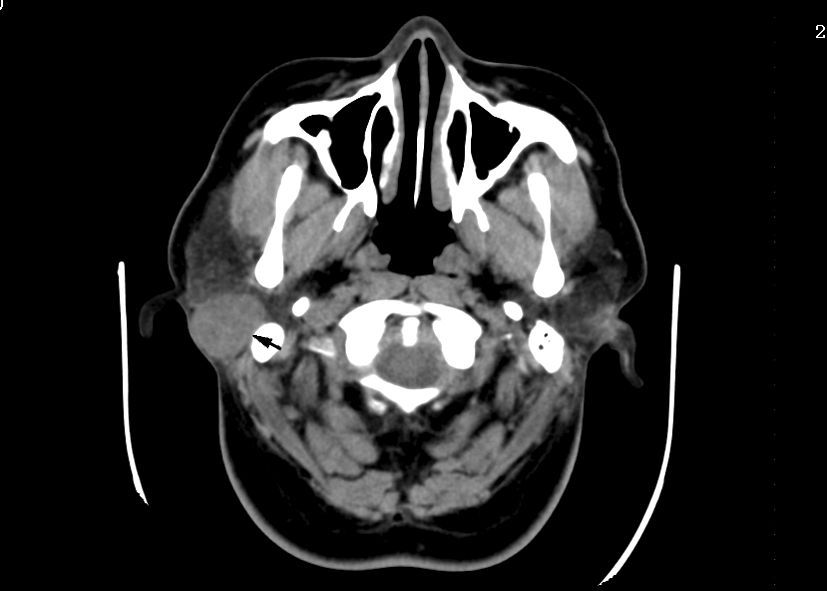
\includegraphics[width=.7\textwidth,height=\textheight,keepaspectratio]{./images/Image00162.jpg}
 \captionsetup{justification=centering}
 \caption{右侧腮腺混合瘤\\{\small 右侧腮腺浅叶区有椭圆形高密度结节,密度欠均匀,界限清晰}}
 \label{fig7-5}
  \end{figure} 

总之,边缘清楚、肿物内部有不同形态的低密度区为良性腮腺混合瘤的特点;肿瘤边界不清、有大片坏死区应考虑恶性混合瘤的可能;长期腮腺肿物病史,近期迅速增大,有助于恶性混合瘤的诊断。

\subsection{涎腺腺淋巴瘤}

本病又称淋巴乳头状囊腺瘤、Warthin瘤,是腮腺第二常见的良性肿瘤,颌下腺少见,鼻咽部偶可发生。约占涎腺良性肿瘤的6%~10%。

\textbf{【病因病理】}
本病与老年人免疫改变有关,吸烟也可能是诱发因素之一。组织学上,由上皮和淋巴样组织组成。瘤内以细胞成分为主,也可有大小不等的囊肿,有薄的包膜。瘤内罕有坏死。

\textbf{【临床表现】}
本病病程长,可达10年。多见于50~70岁男性。因其无症状而就诊时肿瘤多较大,肿瘤边缘光滑、质地中等。

\textbf{【CT表现】}
有时可有双侧肿物(10%)或一侧腺体内多个瘤灶,但相对较少。平扫呈略高密度,通常呈椭圆形或圆形,也可成分叶状或哑铃形,边缘多较清晰,大小变化很大。肿瘤密度不均、囊变区较小(图\ref{fig7-6})。增强后肿瘤常迅速强化;晚期(120秒后)密度下降者占89%,没有肿瘤延迟强化的现象;增强后囊变区显示更著。

\begin{figure}[!htbp]
 \centering
 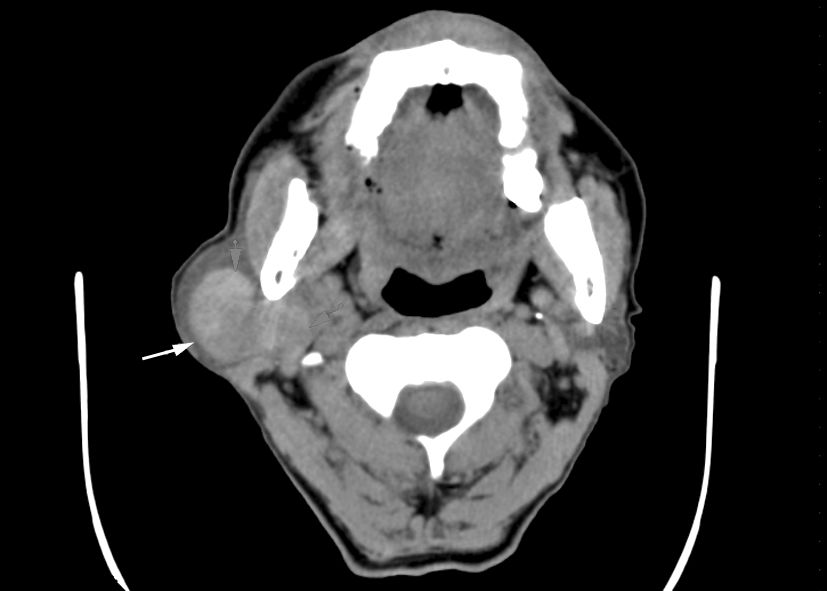
\includegraphics[width=.7\textwidth,height=\textheight,keepaspectratio]{./images/Image00163.jpg}
 \captionsetup{justification=centering}
 \caption{右侧腮腺腺淋巴瘤\\{\small 右侧腮腺区有分叶状稍高密度灶,主要位于浅叶并伸入深叶,边缘清晰,密度欠均}}
 \label{fig7-6}
  \end{figure} 

近期国内有学者认为,50岁以上的男性患者,CT和(或)MR发现腮腺浅叶的后下象限病灶,边界光整,内部密度或信号不均匀,有明显强化,而且多发者,应首先考虑本病可能。

\textbf{【鉴别诊断】}
早期迅速强化、无延迟强化的特点有助于与多形性腺瘤相鉴别。

\section{颞下颌关节疾病}

\subsection{颞下颌关节功能紊乱综合征}

本病又称为颞下颌关节紊乱病,为颞下颌关节最常见的疾病。部分反复发作、经久不愈,严重影响咀嚼功能。

\textbf{【病因】}
①精神因素:可有情绪急躁、易怒、精神紧张,有的有神经衰弱症状;②咬颌关系紊乱:可引起周围肌群的痉挛,并可改变髁状突在关节腔内的正常位置,破坏关节内部正常结构等;③两侧关节发育不对称:造成下颌运动不协调;④单侧咀嚼习惯影响两侧肌肉力量的平衡;⑤关节负荷过重:如经常咀嚼坚硬食物、夜间磨牙等;⑥外伤:寒冷也可以是发病因素。

\textbf{【病理】}
可分为3期:①功能紊乱期:关节区神经肌肉功能紊乱;②结构紊乱期:主要为关节盘移位、关节囊扩张、关节盘和韧带松弛等;③器质性改变期:主要为髁状突的骨、软骨的改变及关节盘破裂、穿孔等。在组织病理学上髁状突、软骨及关节均为典型的退行性变,故认为本征实质上是继发性退行性骨关节病。

\textbf{【临床表现】}
好发于青壮年,以20~30岁最常见,女性为男性的3~5倍。①疼痛,常在咀嚼运动时加重;②关节内弹响或杂音;③运动障碍;④部分患者可伴有患侧头痛、耳鸣、耳痛及颈、肩甚至上肢、腰背的不适。

\textbf{【影像学表现】}
本病的X线平片和体层片、CT、造影检查以及MR检查对器质性破坏期的骨关节改变和结构紊乱期的关节盘、关节囊改变有重要诊断价值。而对功能紊乱期无甚意义,或仅表现为活动异常。对关节盘病变的显示以MR为首选。

1.X线平片及CT平扫表现:①关节间隙的改变:前间隙增宽或变窄,整个间隙变窄或增宽。②骨质改变:髁状突前斜面硬化或模糊毛糙;髁状突凹陷缺损;髁状突前斜面广泛破坏;髁状突囊样变;髁状突骨质增生;髁状突磨平、变短小;关节结节、关节凹硬化。③两侧关节发育不对称。④髁状突运动度的变化。

2.造影表现:一般采用上腔造影法。①上下腔穿通。②关节盘移位:CT可显示位于髁状突和造影剂之间的关节盘的位置。正常时关节盘后带后缘与髁状突横嵴相对应;开口位时关节盘中带与髁状突横嵴相对应。脱离此正常位置即为关节盘移位。a.前移位:闭口位表现为关节盘位于髁状突前斜面的前方。开口位时髁状突向前下方移位,关节盘向后反跳,恢复正常关节盘、髁状突关系,为可复性前移位,否则称为不可复性前移位。b.外移位:较常见。X线闭口位可见关节上腔造影剂边缘“S”形正常形态消失,明显受压变薄或中断。CT可显示移位的关节盘位置。c.旋转移位:较常见。即关节盘前端向内,后端向外的旋转移位,常伴有不同程度的前移位。闭口位表现为“S”型造影剂前部明显聚集,而后部明显变薄,甚至完全消失。③关节囊扩张和松弛:表现为关节腔体积增大和扩张。④关节囊撕裂:可见造影剂外溢。⑤滑膜改变:造影剂边缘不规整,说明有不规则滑膜增生。

\textbf{【鉴别诊断】}
颞下颌关节类风湿性关节炎X线和CT偶见关节间隙增宽,系由于关节周围软组织水肿及滑膜充血增厚所致。软骨破坏后关节间隙变窄甚至消失。髁状突前斜面骨皮质破坏消失、边缘毛糙,有时可见髁状突骨质疏松。仅凭影像学不能明确鉴别颞下颌关节功能紊乱综合征器质破坏期与类风湿性关节炎,须密切结合病史及其他临床检查综合诊断和鉴别。

\subsection{颞下颌关节强直}

本病是由关节本身的病理改变如化脓性关节炎、外伤或类风湿等致病因素的作用而使关节活动丧失,表现为开口困难或完全不能开口。

\textbf{【病理】}
关节结构受到严重破坏,在修复过程中被含有血管的纤维组织所代替,并将破坏的骨性结构愈着、固定在一起,导致纤维强直。这些纤维组织进一步骨化即致骨性强直。

\textbf{【临床表现】}
主要表现为开口困难。纤维性强直患者可以稍有开口活动,而骨性强直患者完全不能开口。儿童时期发生强直者,可影响下颌骨的发育而致小颌畸形。

\textbf{【影像学表现】}
①纤维性强直:髁状突运动受限,骨性结构有不同程度的破坏,形态不规则,关节间隙模糊不清,密度增高。②骨性强直:关节正常的骨结构形态完全消失,关节凹与髁状突出现球形愈合,有时见骨小梁贯穿关节。CT对显示骨性强直的范围优于X线检查。

\subsection{颞下颌关节脱位}

正常颞下颌关节的活动范围是:张口位时髁状突沿关节凹向前弧形滑动至关节结节;闭口位时髁状突又能回复至关节凹内,两侧动度对称。若髁状突超过了上述正常活动范围,且又不能自行回复至关节凹内者,称颞下颌关节脱位。脱位按部位可分为单侧或双侧;按性质可分为急性、复发性和陈旧性;按髁状突脱出的方向、位置可分为前方、后方、上方及侧方脱位。

\textbf{【病因病理】}
急性前脱位常于过大开口时发生。复发性脱位多因急性前脱位处理不当,如复位后未制动或制动时间不够,被撕裂的韧带、关节囊未得到修复而松弛所致。此外,慢性消耗性疾病、肌张力减低、韧带松弛等也可导致复发性脱位。陈旧性脱位患者,髁状突长期脱位于关节结节前上方,致局部组织受撕拉,并有不同程度的结缔组织增生;相应咀嚼肌也会不同程度的痉挛。

\textbf{【临床表现】}
患者常呈开口状,不能闭合。下颌前伸,两颊变平;耳屏前空虚、凹陷,可触及脱位的髁状突。

\textbf{【影像学表现】}
以X线检查为优,但CT诊断医师应对此予以掌握,避免漏诊或误诊。

1.完全性关节脱位:①张口位:髁状突超越关节结节,并位于其前方;②闭口位:髁状突不能回复,仍固定在关节结节的前方(图\ref{fig7-7})。

\begin{figure}[!htbp]
 \centering
 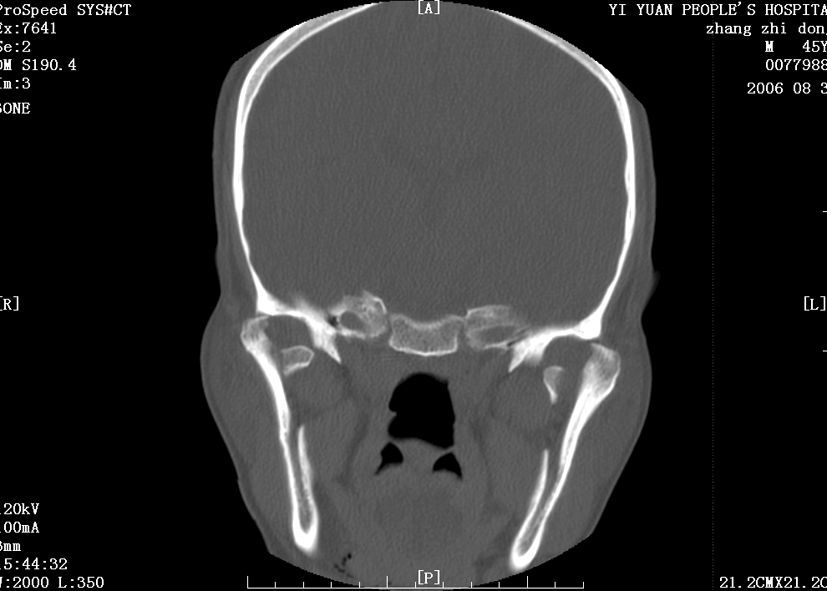
\includegraphics[width=.7\textwidth,height=\textheight,keepaspectratio]{./images/Image00164.jpg}
 \captionsetup{justification=centering}
 \caption{双侧颞颌关节脱位\\{\small 合并髁状突骨折}}
 \label{fig7-7}
  \end{figure} 

2.部分性关节脱位:①张口位:髁状突位于关节结节的前方或前下方;②闭口位:髁状突有部分回复,但仍位于关节结节处、不能完全回复至关节凹内。

3.习惯性脱位:①张口位:髁状突向前超越关节结节;②闭口位:髁状突完全回复到关节凹内。

\subsection{颞下颌关节肿瘤}

颞下颌关节肿瘤并不多见。

\subsubsection{良性肿瘤}

有髁状突骨瘤、骨软骨瘤、滑膜软骨瘤病、滑膜瘤及骨巨细胞瘤等。其中以髁状突骨瘤和骨软骨瘤较多见。

\textbf{【影像学表现】}
髁状突骨瘤和骨软骨瘤表现为骨性突起,可为完全致密性,亦可表现为外有密质骨覆盖、中间松质骨与髁状突相通连(图\ref{fig7-8})。骨软骨瘤表面有明显软骨成分覆盖时,作关节下腔造影时,可见下腔造影剂与髁状突间有一低密度间隙,而髁状突骨瘤则无此表现。滑膜软骨瘤病可见关节腔内有数个大小不一的致密影,髁状突常有不同程度的破坏。关节造影还可发现关节囊扩张、囊壁组织增厚等。

\begin{figure}[!htbp]
 \centering
 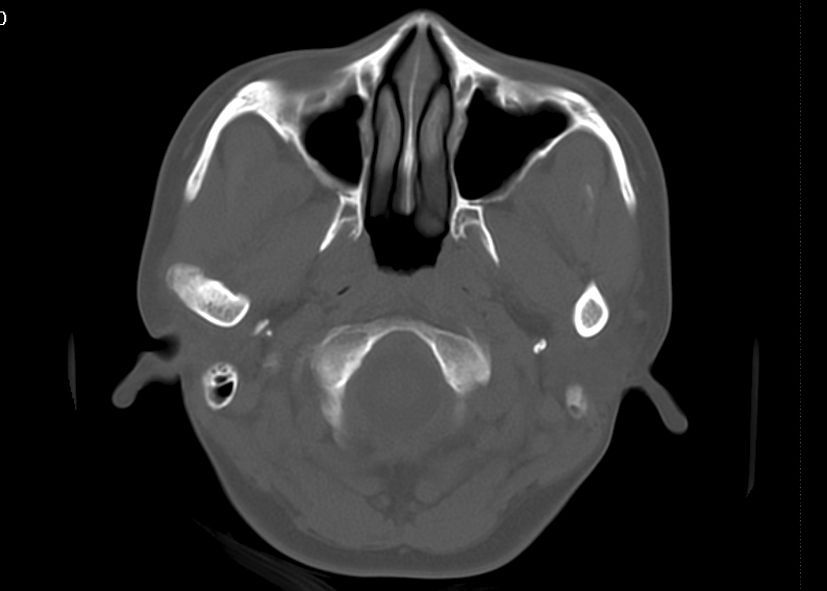
\includegraphics[width=.7\textwidth,height=\textheight,keepaspectratio]{./images/Image00165.jpg}
 \captionsetup{justification=centering}
 \caption{右侧髁状突骨软骨瘤\\{\small 局部有骨性突起,边缘欠光整,有斑点状低密度灶}}
 \label{fig7-8}
  \end{figure} 

\subsubsection{恶性肿瘤}

以转移性肿瘤较常见。原发性以骨肉瘤、滑膜肉瘤及软骨肉瘤相对较常见。

\textbf{【影像学表现】}
早期X线检查可无阳性改变。可见关节骨性结构呈溶骨性明显破坏,邻近可有不规则软组织肿块,严重者侵及颅内和颞下窝。转移瘤主要发生于髁状突,也可同时累及下颌角、下颌升支。

\protect\hypertarget{text00015.html}{}{}

